%%
%%    Short Course on Numerical Modeling in Solid Earth Dynamics
%%    Moresi 
%%

\documentclass[10pt]{article}


\newcommand{\dGamma}{\mathbf{d}\boldsymbol{\Gamma}}
\newcommand{\erfc}{\mbox{\rm erfc}}
\newcommand{\curly}{\sf }
\newcommand{\Red     }[1]{\textcolor[rgb]{0.7,0.0,0.0}{#1}} 
\newcommand{\Green   }[1]{\textcolor[rgb]{0.0,0.7,0.0}{ #1}} 
\newcommand{\Blue    }[1]{\textcolor[rgb]{0.0,0.0,0.7}{ #1}} 
\newcommand{\Emerald }[1]{\textcolor[rgb]{0.0,0.7,0.3}{ #1}} 

\input{../+LaTeX/LectureNotesSetup.tex}

% Different versions of this document ... 
% including answers / example solutions or not

\hideexamplesolutions
\hideanswers
\hideadvanced
\hidelecturehints

% \usepackage{amsmath,amssymb,amstext,epsf,times,colordvi} 


\begin{document}
\title{Numerical Modeling in Solid Earth Dynamics }
\author{Louis Moresi} 
\date{1999-2012}
\maketitle

\section{Introductory Remarks}

	We have considered the application of mathematical reasoning to 
	construct models of the behaviour of physical systems. Unfortunately, most
	of these models do not have analytic solutions or the solutions are so complicated
	that they don't help us understand the problem. The alternative is to solve
	such problems numerically (approximately). Such solutions are also
	possible for far more elaborate systems than we would even consider
	trying to obtain exact solutions for.
	
	On the other hand, numerical modeling only provides solutions to mathematical
	equations and only approximate solutions at that. Unless the modeler has an 
	understanding of the methods and the models themselves, then the output
	of some computer code may be terribly misleading.

	It is always necessary to design a numerical experiment as carefully as
	one would a physical experiment --- although it won't blow up and kill you. 
	It is possible to change the laws of physics in the numerical model often
	inadvertantly, so a careful analysis of the problem first is not a bad idea.
	
	This part of the course contains some really hard material. This is deliberate
	because the workings of most computer codes are actually based on some
	astonishingly intricate mathematics.
	This is really intended to provide a decent reference for people coming back to 
	use finite elements or other numerical methods later. 


\section{Numerical modeling primer}

	We start with the numerical solution of a very simple differential
	equation. In fact we choose something simple enough that we already 
	know the answer.
		\begin{equation}
			\frac{d\theta}{dt} = - k \theta
			\label{eq:ode_decay}
		\end{equation}	
	This is the equation which governs radioactive decay, in which case
	$\theta$ is the amount of the radioactive isotope remaining and $d\theta /  dt$
	is the activity that we can measure. $k$ is closely related to the half life.
	
	The solution to this equation is
		\begin{equation}
			\theta(t) = \theta_0 e^{-kt}
		\end{equation}	
	where $\theta_0$ is the amount of the radioactive material remaining.
	The same equation also describes the cooling of, say, a cup of coffee. In this
	case we interpret $\theta$ as the excess temperature (above room temperature).
	
	%% FIGURE: theta as a function of time 
		\begin{figure}[h]           
			\begin{center}
	 			 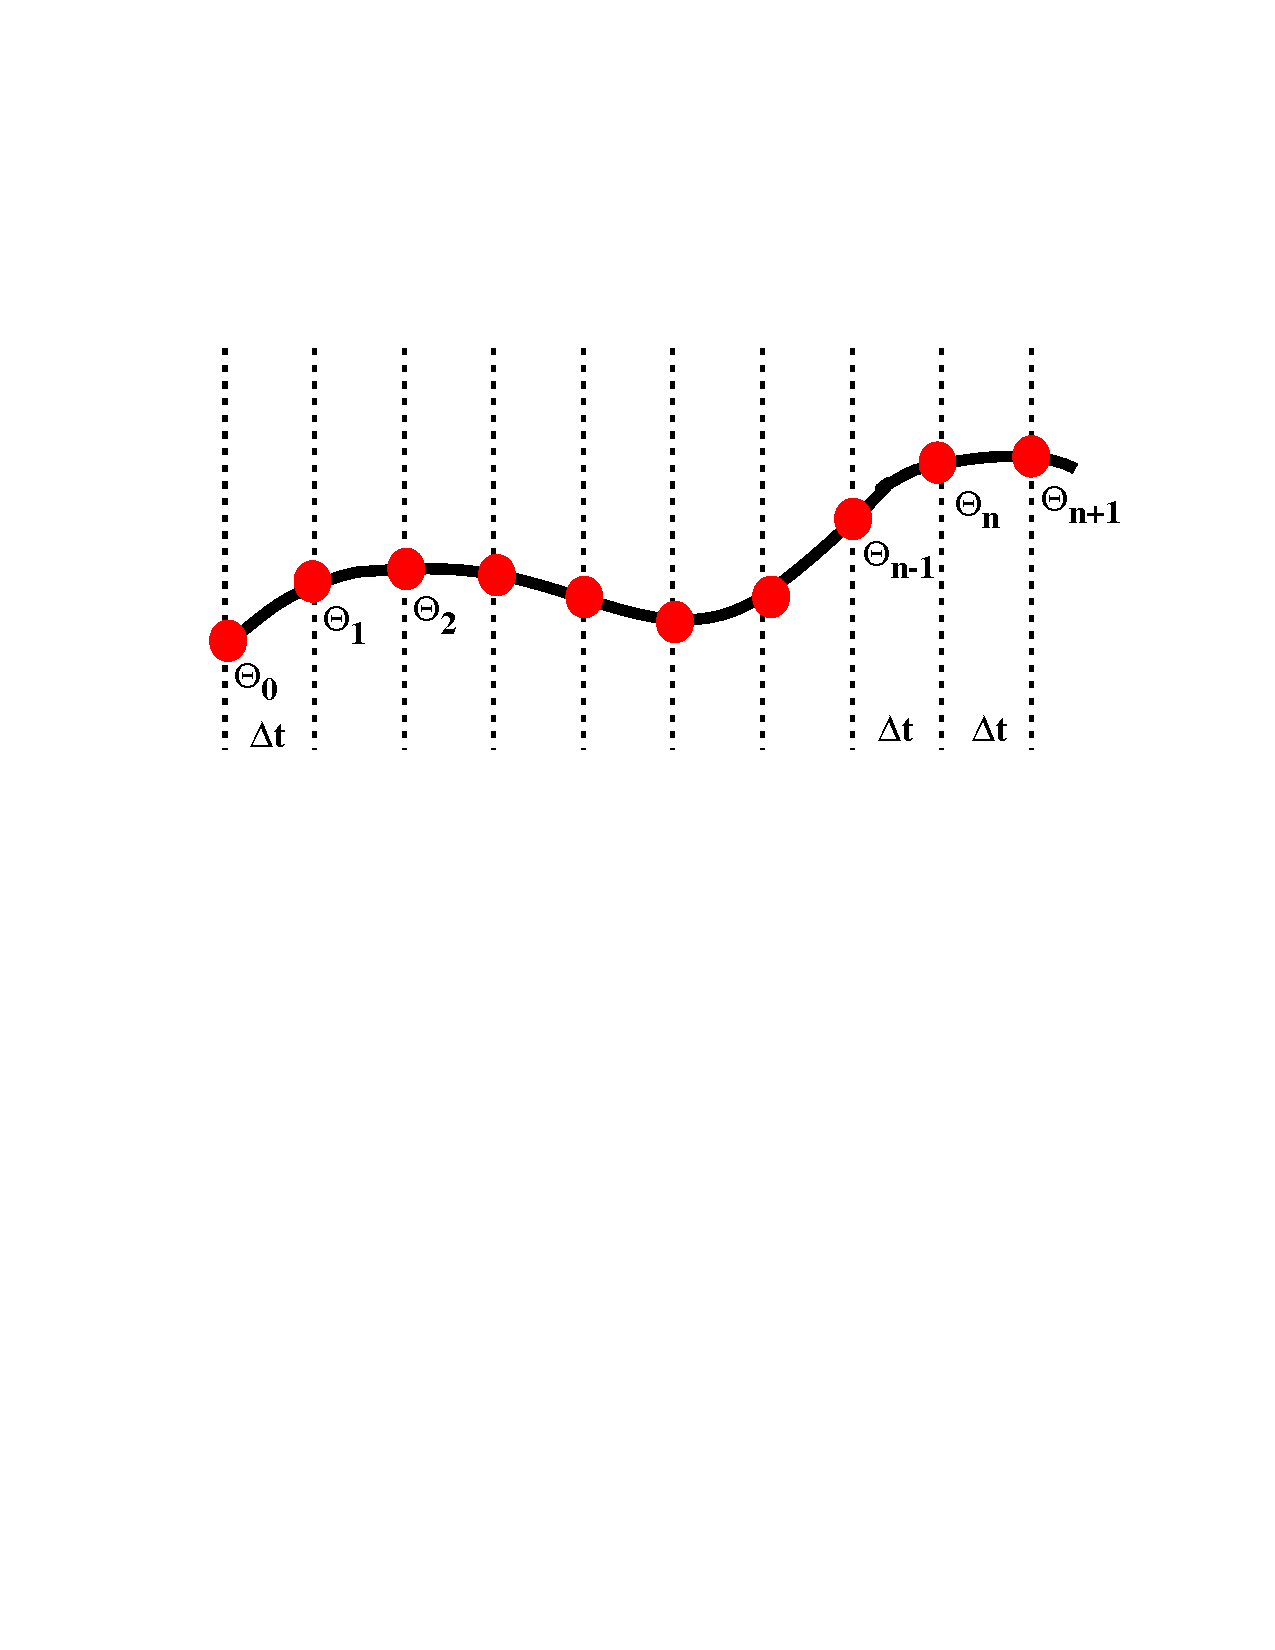
\includegraphics[width=0.66\linewidth]{Diagrams/theta_t.pdf}
	 			\caption[]{Marching through time in small increments}
	 		\end{center}
		\end{figure}
	
	We want to march forward in time from our starting point
	where $\theta = \theta_0$ to obtain the value of $\theta$ at
	later times. To do this, we need to approximate the original
	differential equation, and, in particular, the value of the time
	derivative at each time. There are a number of ways to do this.
	
	\subsection{A first order numerical approximation}
	
	 Assume that the variation in $\theta(t)$ is linear, i.e.
	 	\begin{equation}
	 		\theta(t') = \theta_n + \beta t'
	 	\end{equation}
	 where we use a local time coordinate $t' = t - n\Delta t$, so that
	 when we differentiate
	 	\begin{equation}
	 		\frac{d \theta}{dt} = \beta
	 	\end{equation}
	To determine the approximation for the derivative therefore
	becomes the solution to the following equation:
		\begin{equation}
			\begin{split}
				& \theta_{n+1} = \theta_n + \beta \Delta t \\
				& \Rightarrow	\beta = \frac{d \theta}{dt} = \frac{\theta_{n+1} - \theta_n}{\Delta t}
			\end{split}
		\end{equation}
		
	This is a first order difference expression for the derivative which we
	substitute into the original differential equation (\ref{eq:ode_decay}) at
	the current timestep
	
		\begin{equation}
			\frac{\theta_{n+1} - \theta_n}{\Delta t} = - k \theta_n
		\end{equation}
		
	This rearranges to give us a time-marching algorithm:
	
		\begin{equation}
			\theta_{n+1} = \theta_n (1-k \Delta t)
		\end{equation}
		
	It is an indication of the fact that this problem is really not all that difficult
	that this difference equation can be written recursively
	to give:
		\begin{equation}
			\theta_{n+1} = \theta_0 (1-k \Delta t)^n
		\end{equation}	
	In a moment we will compute some values for this expression to see how
	accurate it is. First we consider whether we can improve the accuracy of the
	approximation by doing a bit more work.
	
	\subsection{Higher order expansion}
	
	First we try fitting the local expansion for $\theta$ through an
	additional point.	 This time we assume that the variation in $\theta(t)$ is quadratic, i.e.
	 	\begin{equation}
	 		\theta(t') = \theta_{n-1} + \beta t' + \gamma {t'}^2
	 	\end{equation}	
	 The local time coordinate is $t' = t - (n-1)\Delta t$, and when
	 we differentiate
	 	\begin{equation}
	 		\frac{d \theta}{dt} = \beta + 2 \gamma t'
	 		\label{eq:dthdt2}
	 	\end{equation}	
	 To solve for $\beta$ and $\gamma$ we fit the curve through
	 the sample points:
	 	\begin{equation}
	 		\begin{split}
	 			\theta_n &= \theta_{n-1} + \beta \Delta t + \gamma (\Delta t)^2 \\
				\theta_{n+1} &= \theta_{n-1} + 2 \beta \Delta t + 4 \gamma (\Delta t)^2
	 		\end{split}
	 	\end{equation}	
	Which solve to give
		 \begin{equation}
		 	\begin{split}
	 			\beta &= \left( 4 \theta_n - \theta_{n+1} - 3\theta_{n-1} \right) \frac{1}{2\Delta t} \\
	 			\gamma &= \left( \theta_{n+1} + \theta_{n-1} -2 \theta_n \right) \frac{1}{2\Delta t^2} 
	 		\end{split}
	 	\end{equation}
	 By substituting into (\ref{eq:dthdt2}), and then into the
	 original differential equation (\ref{eq:ode_decay}) we obtain the following
	 	\begin{equation}	 	
	 			\left. \frac{d\theta}{dt} \right|_{t=n\Delta t} = \beta + 2\gamma \Delta t =
	 				\frac{1}{2\Delta t} \left( \theta_{n+1} - \theta_{n-1} \right)  = -k \theta_n 
	 	\end{equation}
	The difference approximation to the derivative turns out to be the average of the expressions for the
	previous derivative and the new derivative. We have now included information about the current timestep
	and the previous timestep in our expression for the value of $\theta$ at the forthcoming timestep:	
		\begin{equation}
				 \theta_{n+1} = \theta_{n-1} -2k \theta_n \Delta t
		\end{equation}
	
	\subsection{A comparison of the two schemes}
	
	How well do these two methods perform, and what difference does the 
	choice of $\Delta t$ make on the accuracy ?
	
		\begin{table}[h]
		\begin{center}
			\begin{tabular} {r | r r rr r}
				t	& $^1\theta_H$ & $^1\theta_h$ & $^2\theta_H$ & $^2\theta_h$ & Exact \\ \hline
				0.0   &	1.0000  	& 1.0000	& 1.0000 	& 1.0000 	& 1.0000 \\
				0.1	&	---			&	0.9000	& ---			& 0.9000 	& 0.9048 \\
				0.2	& 0.8000	& 0.8100	& 0.8000	& 0.8200 	& 0.8187 \\
				0.3 	& ---     		& 0.7290	& ---			&	0.7360	&	0.7408 \\
				0.4	& 	0.6400	& 0.6561	& 0.6800	& 0.6728	& 0.6703 \\
				0.5	& ---			& 0.5905	& ---			& 0.6014	& 0.6063 \\
				0.6	& 0.5120	& 0.5314	& 0.5280	& 0.5525	& 0.5488 \\
				0.7	& ---			& 0.4783	& ---			& 0.4909	& 0.4966 \\
				0.8	& 0.4096	& 0.4305	& 0.4688	& 0.4543	& 0.4483 \\
				0.9	& ---			& 0.3874	& ---			& 0.4001	& 0.4066 \\
				1.0	& 0.3277	& 0.3487	& 0.3405	& 0.3743	& 0.3679
			\end{tabular}	
		\end{center}	
		\caption[]{Results of the numerical simulation of the decay equation. $^1\theta_H$ is from the
		 first order expansion of $\theta(t)$, at a timestep of $\Delta t=0.2$, and $^2\theta_H$ is
		 the second order expansion at $\Delta t=0.2$; other calculations are at $\Delta t = 0.1$. 
		$^1\theta_h$ is the linear expansion,  $^2\theta_h$ results from the quadratic expansion
		of $\theta(t)$. The actual solution is also shown.}
		\end{table}
	  
	The results are more accurate when a smaller timestep is used although it
	requires more computation to achieve the greater accuracy. Higher order expansion
	also increases the accuracy and may be more efficient in terms of the number of computations
	required for a given level of accuracy.
	
	Note, however, that the supposedly better quadratic expansion produces an error which
	oscillates as time increases. Does this error grow ? Does this make second order
	expansions useless ?
	
		\subsection{Second Order Runge-Kutta}
	
	%% FIGURE: theta as a function of time 
		\begin{figure}[h]           
			\begin{center}
	 			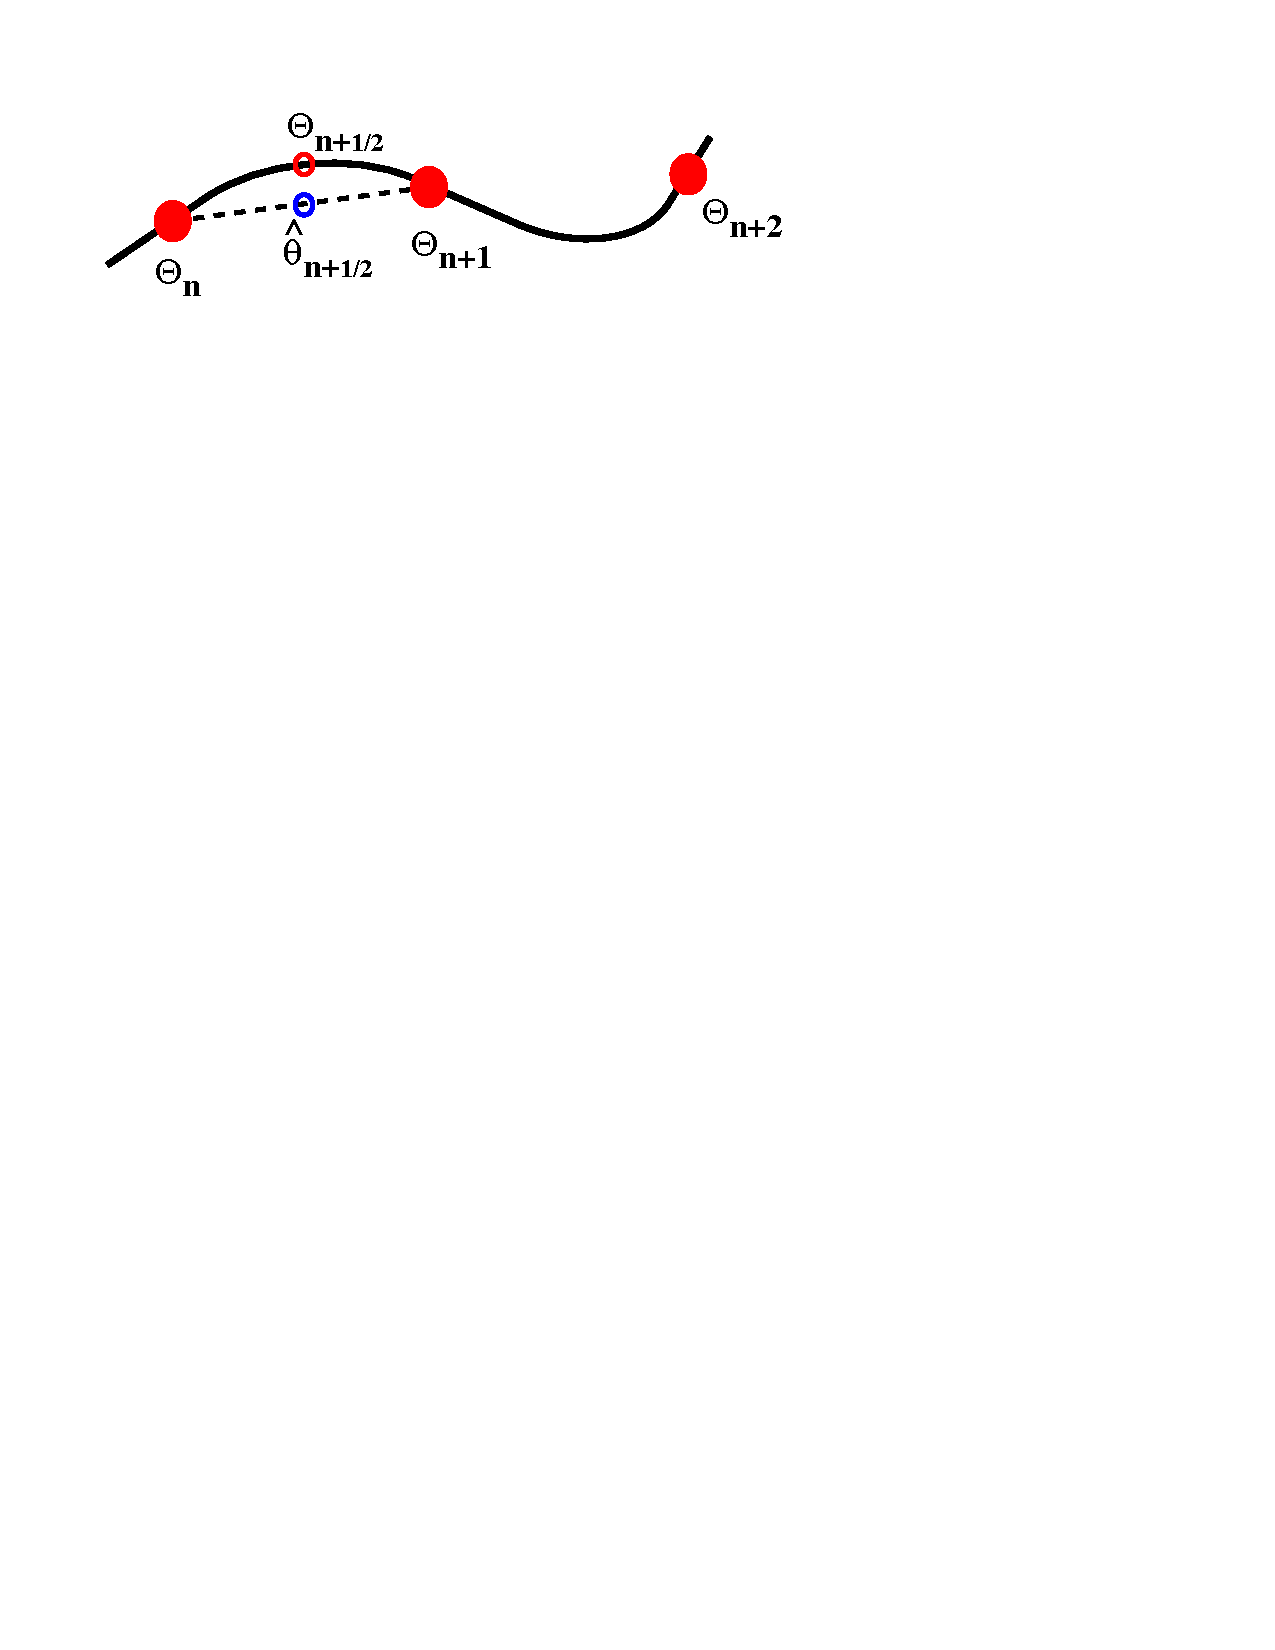
\includegraphics[width=0.66\linewidth]{Diagrams/theta_rk2.pdf}
	 			\caption[]{A different way to get a second order method}
	 			\label{fig:rk2}
	 		\end{center}
		\end{figure}
	
	The Runge-Kutta approach to higher order integration methods is
	illustrated in Figure \ref{fig:rk2}. The idea is to estimate the 
	gradient $d \theta / d t$ at the half way point between two
	timestep values.  This is done in two stages. Initially a 
	first order estimate, $\hat{\theta}$ is made for the value of the function
	$\theta$ at $t=t+\Delta t /2$ in the future. This value is then
	subsituted into the differential equation to obtain the
	estimate for the gradient at this time. The revised gradient is
	then used to update the original $\theta(t)$ by an entire timestep.
	
	The first order step is
		\begin{equation}
			\begin{split}
				\hat{\theta}(t+\Delta t /2) & = \theta(t) + \left.  \frac{d \theta}{d t} \right|_t \frac{\Delta t}{2} \\
					&= \theta(t) \left[ 1-\frac{k\Delta t}{2} \right]
			\end{split}
		\end{equation}
	Substitute to estimate the gradient at the mid-point
		\begin{equation}
			 \left. \frac{d \theta}{d t} \right|_{t+\Delta t /2} \approx -k \theta(t)  \left[ 1-\frac{k\Delta t}{2} \right]
		\end{equation}
	Use this value as the average gradient over the interval $t\rightarrow t+\Delta t$ to
	update $\theta$
		\begin{equation}
			\begin{split}
				\theta(t+\Delta t) & \approx \theta(t) + \delta t \left(  -k \theta(t)  \left[ 1-\frac{k\Delta t}{2} \right]  \right) \\
					& \approx \theta(t) \left( 1 - k \Delta t + k^2 \frac{\Delta t^2}{2} \right)
			\end{split}
		\end{equation}
	It's worth noting that the Taylor expansion of the solution should look like
		\begin{equation}
			e^{-kt} = 1 - kt + \frac{k^2 t^2}{2!} - \frac{k^3 t^3}{3!} + \ldots
		\end{equation}
	
	The Runge Kutta method can be extended by repeating the estimates on smaller regions of the interval.
	The usual choice is fourth order RK. This is largely because, obviously, it's accurate to fourth order, but also because
	the number of operations to go higher than fourth order is disproportionately large. See
	Numerical Recipes for a discussion on this and better methods for ODE's.
	
		
	\subsection{Our First Code}
	
	The simplest way to answer our earlier question is to code the
	methods and see. The following is a PERL script which computes the first and second 
	order expressions and the Runge-Kutta method, and compares with the `exact' solution
	(which is numerical as well, of course, but computed through series expansions and
	the like).
	
	{\footnotesize
		\begin{verbatim}
		#! /usr/local/bin/perl
		
		# Compare various ways to integrate the 
		# ODE for radioactive decay / Newton's law of cooling.
		# Assume decay constant of 1.0
		
		$timestep=0.1;
		
		# Initial value ... 
		
		$theta1_0   = 1.0;
		$theta2_0   = 1.0;
		$thetaRK2_0 = 1.0;
		
		# First timestep (by hand, then automate for subsequent cases)
		
		$theta1_1   = 0.9;
		$theta2_1   = 0.9;
		$thetaRK_1  = 0.905;
		
		# Now we have enough information to automate all the methods 
		
		for($i=2;$i<=1000;$i++) {
		
		  $time = $timestep * $i;
		  $exact = 1.0 * exp(-1.0 * $time);
		
		  $theta1_2 = $theta1_1 * (1.0 - $timestep);
		  $theta2_2 = $theta2_0 - 2.0 * $theta2_1 * $timestep;
		  $thetaRK_2 = $thetaRK_1 * (1.0 - $timestep + 0.5 * $timestep * $timestep);
		
		  # output data every 25th step
		  if(! ($i % 25)) {
		    printf "Timestep %04d (%f)\t %.4e \t %.4e \t %.4e \t %.4e \n",
		    			$i,$time,$theta1_2,$theta2_2,$thetaRK_2,$exact;
		  }
		
		  # keep old values (not all are needed, of course)
		
		  $theta1_0  = $theta1_1;
		  $theta2_0  = $theta2_1;
		  $thetaRK_0 = $thetaRK_1;
		
		  $theta1_1  = $theta1_2;
		  $theta2_1  = $theta2_2;
		  $thetaRK_1 = $thetaRK_2;
		}
		
		
		# Timestep 0025 (2.5000000)	 7.1790e-02 	  5.2117e-02 	 8.2455e-02 	 8.2085e-02
		# Timestep 0050 (5.0000000)	 5.1538e-03 	  3.7201e-01 	 6.7987e-03 	 6.7379e-03 
		# Timestep 0075 (7.5000000)	 3.6999e-04 	 -4.4304e+00 	 5.6059e-04 	 5.5308e-04 
		# Timestep 0100 (10.000000)	 2.6561e-05 	  5.3757e+01 	 4.6223e-05 	 4.5400e-05 
		# Timestep 0125 (12.500000)	 1.9068e-06 	 -6.5219e+02 	 3.8113e-06 	 3.7267e-06 
		# Timestep 0150 (15.000000)	 1.3689e-07 	  7.9124e+03 	 3.1426e-07 	 3.0590e-07 
		# Timestep 0175 (17.500000)	 9.8274e-09 	 -9.5993e+04 	 2.5912e-08 	 2.5110e-08 
		# Timestep 0200 (20.000000)	 7.0551e-10 	  1.1646e+06 	 2.1366e-09 	 2.0612e-09 
		# Timestep 0225 (22.500000)	 5.0648e-11 	 -1.4129e+07 	 1.7617e-10 	 1.6919e-10 
		# Timestep 0250 (25.000000)	 3.6360e-12 	  1.7141e+08 	 1.4526e-11 	 1.3888e-11 
		# Timestep 0275 (27.500000)	 2.6103e-13 	 -2.0796e+09 	 1.1977e-12 	 1.1400e-12 
		# Timestep 0300 (30.000000)	 1.8739e-14 	  2.5230e+10 	 9.8758e-14 	 9.3576e-14 
		# Timestep 0325 (32.500000)	 1.3453e-15 	 -3.0609e+11 	 8.1431e-15 	 7.6812e-15 
		# Timestep 0350 (35.000000)	 9.6578e-17 	  3.7135e+12 	 6.7143e-16 	 6.3051e-16 
		# Timestep 0375 (37.500000)	 6.9333e-18 	 -4.5052e+13 	 5.5363e-17 	 5.1756e-17 
		# Timestep 0400 (40.000000)	 4.9774e-19 	  5.4658e+14 	 4.5649e-18 	 4.2484e-18 
		# Timestep 0425 (42.500000)	 3.5733e-20 	 -6.6311e+15 	 3.7640e-19 	 3.4873e-19 
		# Timestep 0450 (45.000000)	 2.5652e-21 	  8.0449e+16 	 3.1036e-20 	 2.8625e-20 
		# Timestep 0475 (47.500000)	 1.8416e-22 	 -9.7602e+17 	 2.5590e-21 	 2.3497e-21 
		# Timestep 0500 (50.000000)	 1.3221e-23 	  1.1841e+19 	 2.1100e-22 	 1.9287e-22 
		# Timestep 0525 (52.500000)	 9.4911e-25 	 -1.4366e+20 	 1.7398e-23 	 1.5832e-23 
		# Timestep 0550 (55.000000)	 6.8137e-26 	  1.7429e+21 	 1.4346e-24 	 1.2996e-24 
		# Timestep 0575 (57.500000)	 4.8915e-27 	 -2.1144e+22 	 1.1829e-25 	 1.0668e-25 
		# Timestep 0600 (60.000000)	 3.5116e-28 	  2.5653e+23 	 9.7532e-27 	 8.7565e-27 
		# Timestep 0625 (62.500000)	 2.5210e-29 	 -3.1122e+24 	 8.0420e-28 	 7.1878e-28 
		# Timestep 0650 (65.000000)	 1.8098e-30 	  3.7757e+25 	 6.6310e-29 	 5.9001e-29 
		# Timestep 0675 (67.500000)	 1.2993e-31 	 -4.5807e+26 	 5.4675e-30 	 4.8431e-30 
		# Timestep 0700 (70.000000)	 9.3273e-33 	  5.5574e+27 	 4.5082e-31 	 3.9754e-31 
		# Timestep 0725 (72.500000)	 6.6961e-34 	 -6.7423e+28 	 3.7172e-32 	 3.2632e-32 
		# Timestep 0750 (75.000000)	 4.8071e-35 	  8.1797e+29 	 3.0650e-33 	 2.6786e-33 
		# Timestep 0775 (77.500000)	 3.4510e-36 	 -9.9237e+30 	 2.5273e-34 	 2.1988e-34 
		# Timestep 0800 (80.000000)	 2.4775e-37 	  1.2040e+32 	 2.0838e-35 	 1.8049e-35 
		# Timestep 0825 (82.500000)	 1.7786e-38 	 -1.4606e+33 	 1.7182e-36 	 1.4815e-36 
		# Timestep 0850 (85.000000)	 1.2768e-39 	  1.7721e+34 	 1.4167e-37 	 1.2161e-37 
		# Timestep 0875 (87.500000)	 9.1663e-41 	 -2.1499e+35 	 1.1682e-38 	 9.9824e-39 
		# Timestep 0900 (90.000000)	 6.5805e-42 	  2.6082e+36 	 9.6321e-40 	 8.1940e-40 
		# Timestep 0925 (92.500000)	 4.7241e-43 	 -3.1643e+37 	 7.9421e-41 	 6.7261e-41 
		# Timestep 0950 (95.000000)	 3.3914e-44 	  3.8390e+38 	 6.5486e-42 	 5.5211e-42 
		# Timestep 0975 (97.500000)	 2.4347e-45 	 -4.6575e+39 	 5.3996e-43 	 4.5320e-43 
		# Timestep 1000 (100.00000)	 1.7479e-46 	  5.6505e+40 	 4.4522e-44 	 3.7201e-44 
		\end{verbatim}
	}   %% end of reduced font size
	
	Clearly, the quadratic expansion does not do a good job in this particular case, since
	the error is a growing instability which makes the solution useless almost immediately.
	However, the second order Runge-Kutta method is very accurate. 
	This gives a clear warning that numerical solution of equations is partly an 
	art. 
	

\section{Explicit versus Implicit Methods}

	The use of implicit solution methods is crucial when we come to the 
	mantle flow problem (and to elasticity). It is a deceptively simple concept
	which we use to eliminate oscillatory errors and other problems associated
	with `stiff' systems, and in other cases where we want to take large timesteps.
	Again, Numerical Recipes provides a good example of the way in which
	implicit methods avoid the shuffling timesteps which result when an otherwise
	unimportant component of the system blows up.

	To obtain an implicit solution, we express our updated timestep in terms of
	values of derivatives etc which are evaluated at that timestep. This may 
	result in dependencies which mean large systems of simultaneous equations
	need to be solved. 
	
	But our simple example can also be solved implicitly as follows
		\begin{equation}
			\theta(t+\Delta t) = \left. \frac{d \theta}{d t} \right|_{t+\Delta t} + \theta(t)
		\end{equation}	
	Easy to write down, but $\left. d \theta/ dt \right|_{t+\Delta t}$ is not known  until $\theta(t+\Delta t)$
	is known. In this case, however, we simply substitute $\left. d \theta/ dt \right|_{t+\Delta t}= -k \theta(t+\Delta t)$
	from the differential equation and write
		\begin{equation}
			\begin{split}
				\theta(t+\Delta t)  & = -k \theta(t+\Delta t) \Delta t + \theta(t) \\
												& = \frac{\theta(t) }{ 1 + k\Delta t}
			\end{split}
		\end{equation}

	A higher order implicit method can be found by considering how the second order
	Runge-Kutta method constructs its estimates. In place of the first order
	approximation above, we try
		\begin{equation}
			\theta(t+\Delta t) = \left. \frac{d \theta}{d t} \right|_{t+\Delta t/2} + \theta(t)
		\end{equation}	
	where we assume
		\begin{equation}
			\left. \frac{d \theta}{d t} \right|_{t+\Delta t/2} = 
				\frac{1}{2} \left. \frac{d \theta}{d t} \right|_{t+\Delta t} + 
				\frac{1}{2} \left. \frac{d \theta}{d t} \right|_{t} 
		\end{equation}
	Substituting from our original differential equation now gives
		\begin{equation}
			\begin{split}
				\theta(t+\Delta t) &= -k\frac{\theta(t+\Delta t) + \theta(t)}{2} \Delta t + \theta(t) \\
							&= \theta(t) \frac{1-k\Delta t / 2}{1+k\Delta t / 2}
			\end{split}
		\end{equation}	

	
	%% table for results of implicit scheme
		\begin{table}[h]
			\begin{center}
				\begin{tabular} {r | r r r}
					t	& $^1\theta_i$ & $^2\theta_i$ & Exact \\ \hline
					0.0   & 1.0000 & 1.0000	& 		1.0000 \\
					0.1	& 0.9091	& 0.9048 & 	0.9048 \\
					0.2	& 0.8264	& 0.8186 & 	0.8187 \\
					0.3   & 0.7513	&	0.7406 &	0.7408 \\
					0.4	 & 0.6830	& 0.6701 & 	0.6703 \\
					0.5	& 0.6209	& 0.6063 & 	0.6063 
				\end{tabular}	
			\caption[]{Results of the two implicit schemes derived above for the numerical
			integration of the decay equation}
			\end{center}
		\end{table}
	  
	The first order scheme is of approximately the same accuracy as the
	explicit scheme, not surprisingly, but the mid-point implicit method has 
	very impressive results considering that there is very little
	extra work involved in deriving the formulation.

	Can this strategy stabilize the quadratic expansion which
	proved to be so unstable in explicit form ?
	Evaluating the derivatives at time $t=(n+1)\Delta t$ gives
		\begin{equation}
			\left. \frac{d \theta}{d t} \right|_{(n+1)\Delta t} = 3 \theta_{n+1} - 4\theta_n + \theta_{n-1}	
		\end{equation}
	which we substitute into the differential equation at $t=(n+1)\Delta t$ to
	give (eventually)
		\begin{equation}
			\theta_{n+1} = \frac{4\theta_n - \theta_{n-1}}{3+2k\Delta t}
		\end{equation}
	
	This method is stable although not as accurate as the 
	second order Runge-Kutta Scheme. It is trivial to modify the
	PERL script to demonstrate this.	

\section{Generalizing from the Simplest Example}
 We have learned a number of things --- in particular
 
\begin{itemize}

		\item We have to know something about the governing
		equations of the system before modeling can proceed (i.e. a 
		conceptual model, and then a mathematical model).

	\item Before the equations can be solved in the computer, it is
		necessary to render the problem finite.
			
	\item 
		The discretization method chosen may not be effective for a particular
		problem. Numerical modeling can be an art since experience with different
		differential equations is often needed to avoid pitfalls.
	
\end{itemize}


\section{The Problem with Advection}	

	Advection is a fundamental concept in fluid mechanics, get it makes
	the lives of fluid dynamicists much more difficult. It can be particularly
	problematic in numerical modeling. This is worth having in 
	mind when we discuss different numerical methods because
	in application to solid Earth dynamics, advection will be a major
	issue with any method we choose.
	
	%% FIGURE: theta as a function of time 
		\begin{figure}[h]           
			\begin{center}
	 			 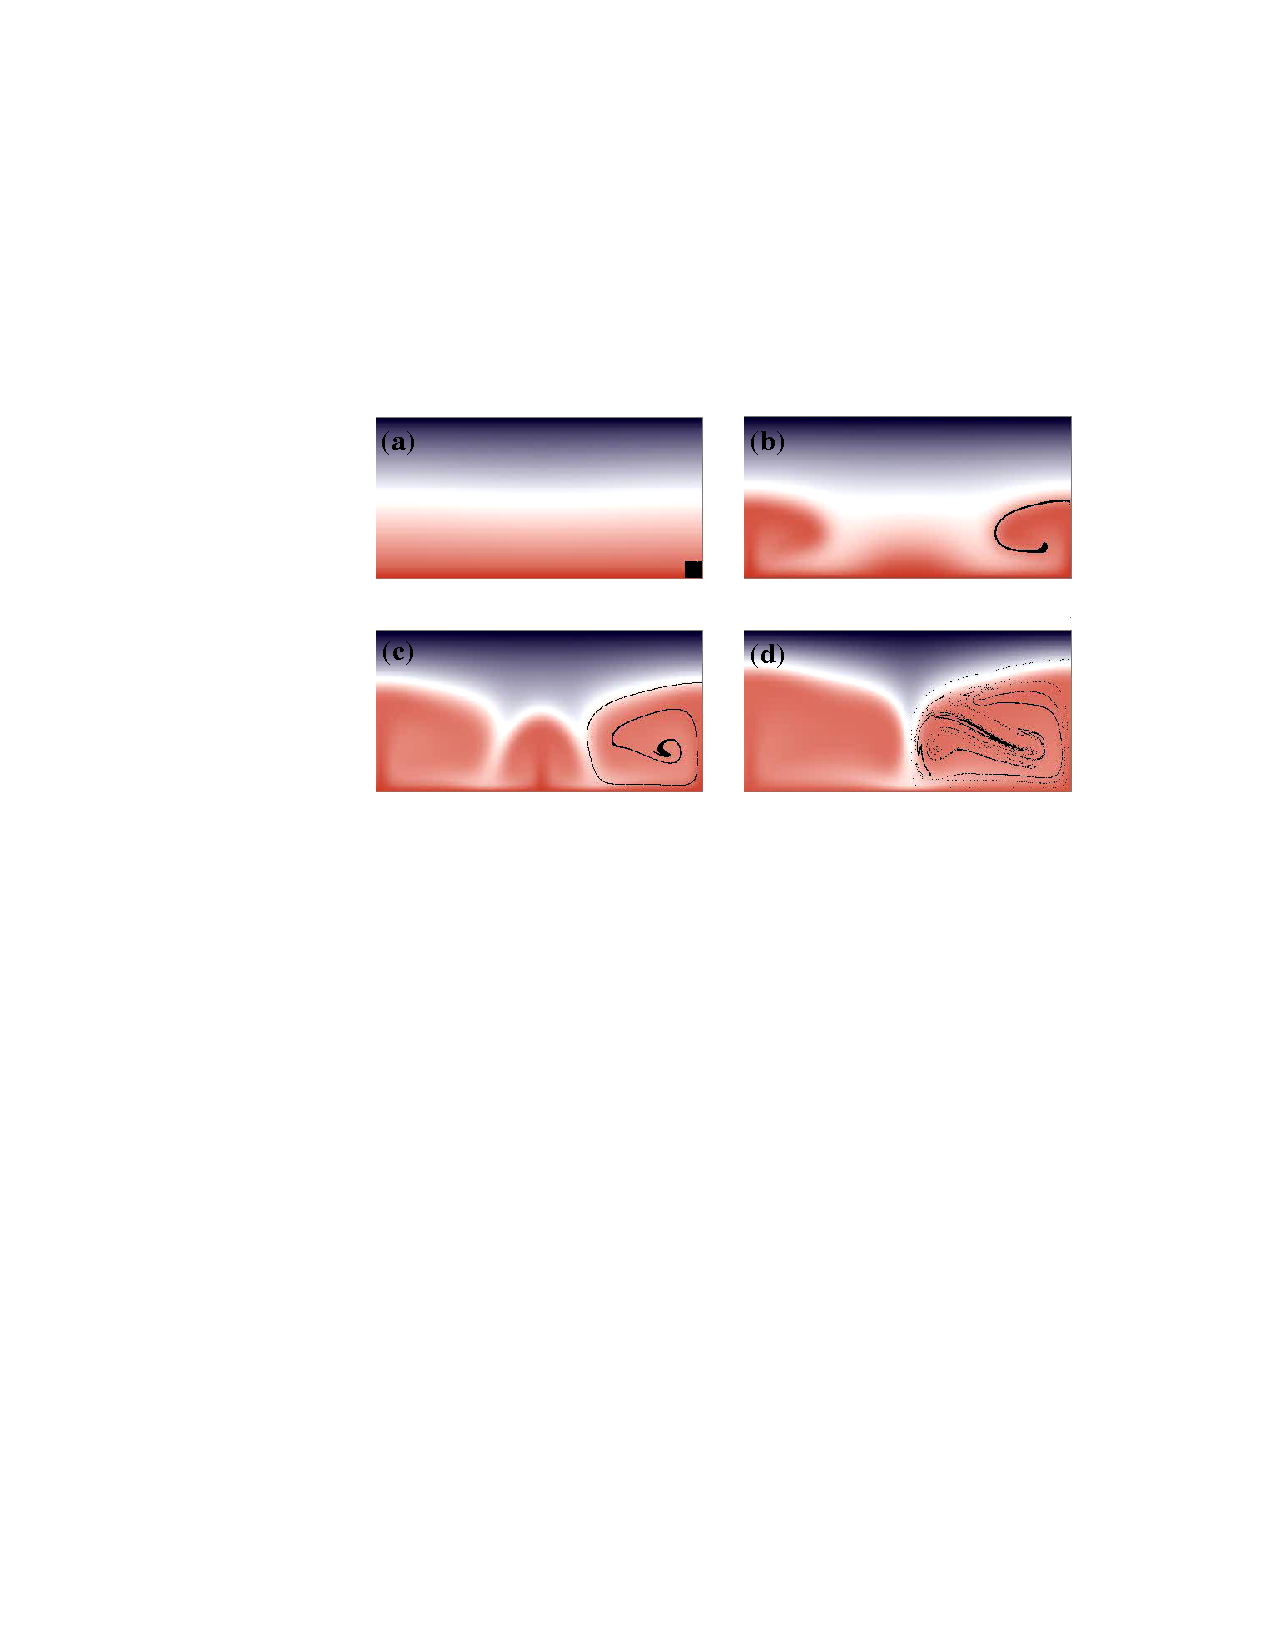
\includegraphics[width=0.66\linewidth]{Diagrams/advect_mix.pdf}
	 			\caption[]{Advection pure and simple --- with no diffusion, fluid
	 			motion winds up initially local regions into long, convoluted tendrils}
	 			\label{fig:adv1}
	 		\end{center}
		\end{figure}
		
	As we discussed in dealing with approximate analytic solutions in Part I, the
	solution to all our advection woes is to deal with a coordinate system locked to 
	the fluid.
	
	Unfortunately, while this approach works well in some situations -- predominantly solid
	mechanics and engineering applications where total deformation is generally no more
	than a few percent strain -- in fluids, the local coordinate system becomes quite
	hard to follow. In figure \ref{fig:adv1}, a small, square region of fluid has been tagged
	and is followed during the deformation induced by a simple convection roll.
	It is clear that a coordinate system based on initially orthogonal sets of axes 
	rapidly becomes unrecognizably distorted. 

	Advection, in the absence of any diffusion terms, represents a transport of information
	about the state of an individual parcel of fluid which is different from the state of its neighbours.
	For example, it might be a dye which tells us whether a parcel of fluid started in
	on half of the domain or the other. 
	We are dealing with a chaotic system in the sense that parcels of material which start abitrarily close
	together will wind up exponentially far apart as time progresses. Thus, the dye
	will become ever more stretched and filamented without ever being mixed (at least in 
	laminar flow).    
	
	If the dye can diffuse then, the finer scales of the tendrils will in fact be mixed
	because they are associated with enormous spatial gradients (e.g. compare this
	with boundary layers). 
	
	If the dye cannot diffuse then the density of information needed to characterize the 
	system increases without limit. Numerically this is impossible to represent since
	at some stage, the stored problem has to be kept finite.  This can be
	imagined as an effective diffusion process, although it has an anisotropic and
	discretization dependent form.  The rule of thumb, that arises from this observation
	is that the {\em real} diffusion coefficient must be larger than the numerical one
	if the method is to give a true representation of the problem. 
	
	\subsection{Numerical Example in 1D}
	
		%% FIGURE: theta as a function of time 
		\begin{figure}[h]           
			\begin{center}
	 			 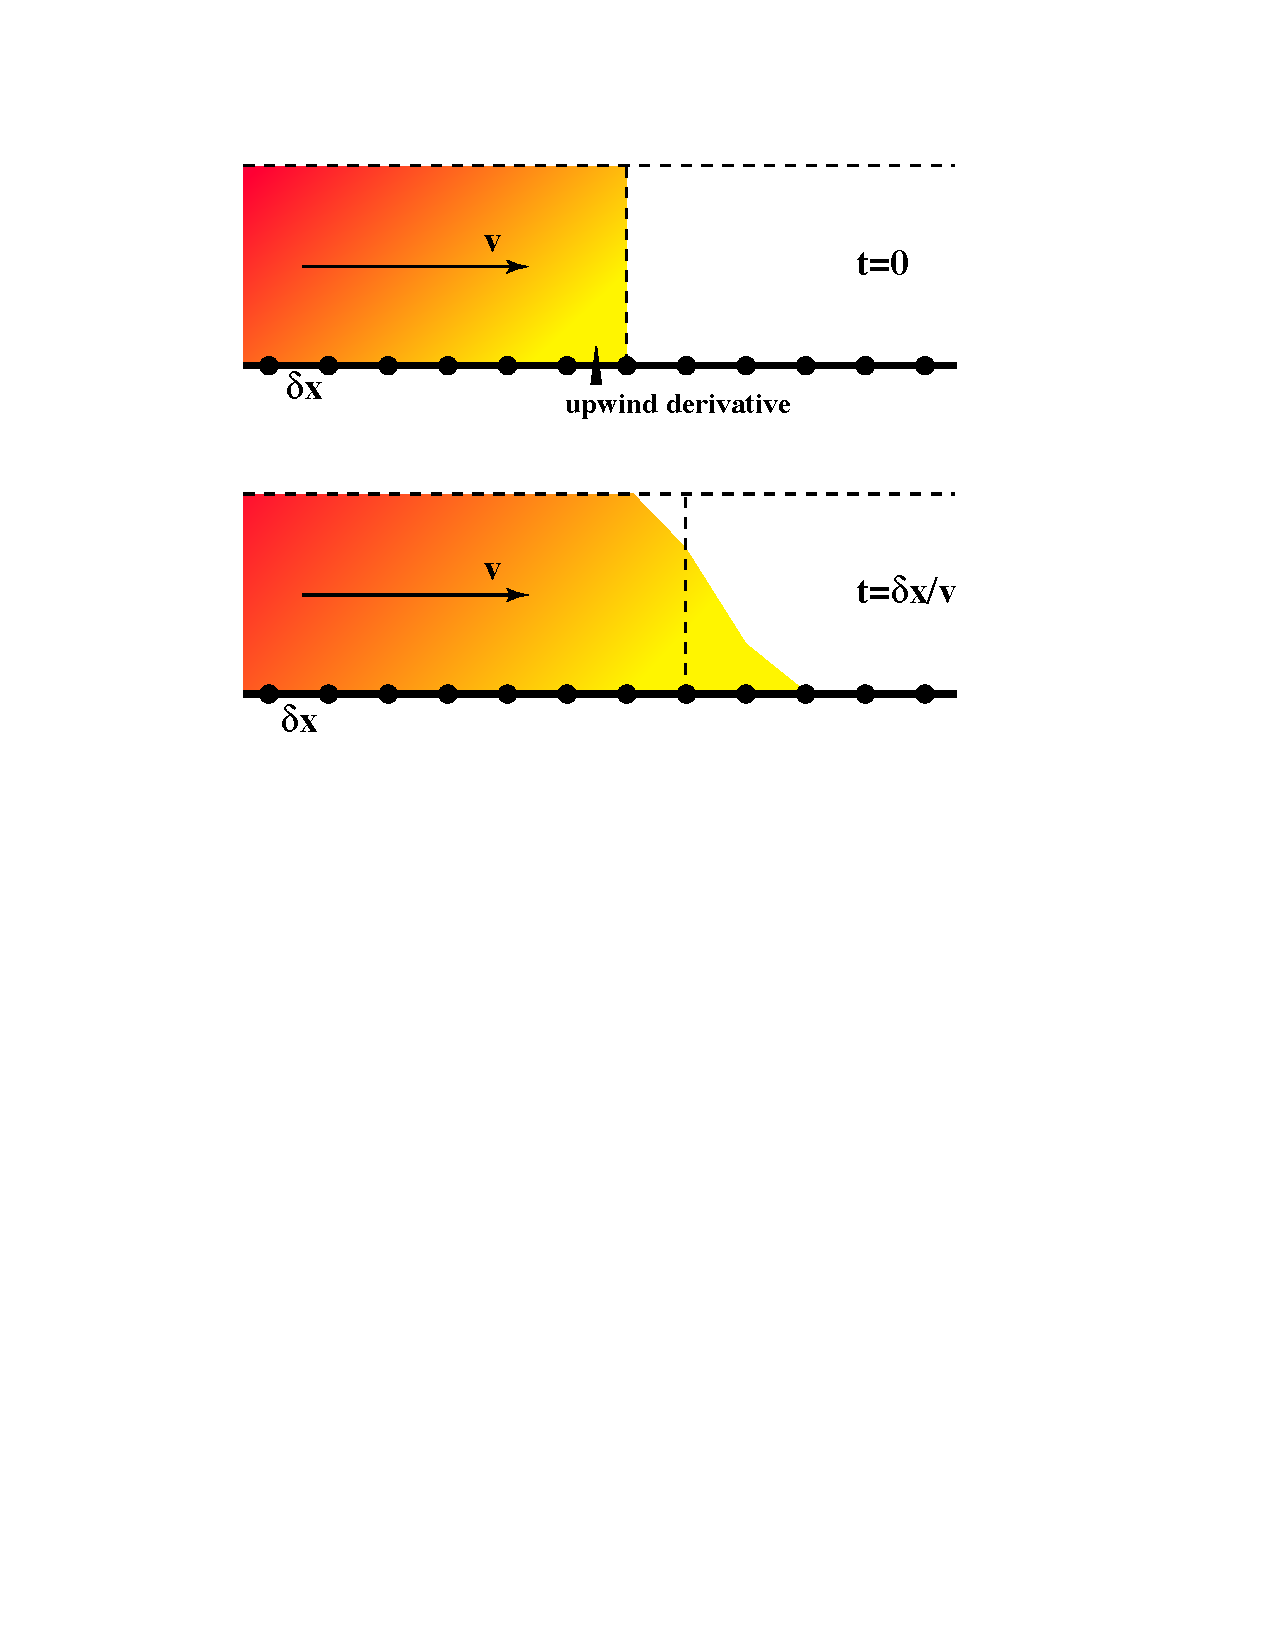
\includegraphics[width=0.66\linewidth]{Diagrams/eul_adv.pdf}
	 			\caption[]{Setup for a first attempt at a numerical advection scheme on
	 				a fixed discretization. After two timesteps, the sharp front has become
	 				smoothed despite introducing no genuine diffusion}
	 			\label{fig:adv2}
	 		\end{center}
		\end{figure}
		
	Let us follow our usual strategy an solve the simplest imaginable advection equation:
		\begin{equation}
			\frac{\partial \phi}{\partial t} = -v \frac{\partial \phi}{\partial x}
		\end{equation}
	in which $v$ is a constant velocity. Obviously we need to introduce some
	notation as a warm-up for solving the problem. We break up the
	spatial domain into a series of points separated by $\delta x$ as 
	shown in Figure \ref{fig:adv2} and, as we did in the earlier examples,
	break up time into a discrete set separated by $\delta t$.
	
	The values of $\phi$ at various times and places are denoted by
		\begin{align}
			&&	&_{i-1}\phi_{n-1}	&&_{i}\phi_{n-1} 	&& _{i+1}\phi_{n-1} && \nonumber \\
			&&	&_{i-1}\phi_{n} 		&&_{i}\phi_{n} 		&& _{i+1}\phi_{n}  &&\\
			&&	&_{i-1}\phi_{n+1}	&&_{i}\phi_{n+1} 	&& _{i+1}\phi_{n+1} &&\nonumber 
		\end{align}
	where the $i$ subscript is the $x$ position and $n$ denotes the timestep:
		\begin{equation}
			\phi(x_i,n\Delta t) = {_{i}\phi}_n
		\end{equation}
	
	A simple discretization gives
		\begin{equation}
			\begin{split}
			_{i}\phi_{n+1} &= \frac{\partial \phi}{\partial t} \Delta t + {_{i}\phi_n} \\
						& = -v \frac{{_{i+1}\phi_n} - {_{i-1}\phi_n}}{2 \delta x} + {_{i}\phi_n}
			\end{split}
		\end{equation}
	For simplicity, we set $v\delta t = \delta x /2$ and write
		\begin{equation}
			{_{i}\phi}_{n+1} = \frac{1}{4}\left(  {_{i+1}\phi}_n - {_{i-1}\phi}_n \right)
		\end{equation}
		
	\begin{table}
		\begin{center}
			\begin{tabular}{l | l | c c c c c c | c}
			\multicolumn{2}{c|}{ }	 & \multicolumn{6}{c|}{location} & \\ 
			& time & i-2 & i-1 & i & i+1 & i+2 & i+3 & $\int \phi dx$ \\ \hline \hline
			Centred & t=0 & 1 & 1 & 1 & 0  & 0 & 0 & 3		\\
				& t=$\delta x/2v$ &  1 & 1 & 1.25 & 0.25  & 0 & 0 & 3.5		\\
				& t=$\delta x/v$ & 1 & 0.938 & 1.438 & 0.563 & 0.0625 & 0 & 4.0 \\ \hline
			Upwind &  t=0 & 1 & 1 & 1 & 0  & 0 & 0 &  3		\\
				& t=$\delta x/2v$ &  1 & 1 & 1 & 0.5  & 0 & 0 & 3.5		\\
				& t=$\delta x/v$ &  1 & 1 & 1 & 0.75  & 0.25 & 0 & 4.0		\\ \hline
			\end{tabular}
		\end{center}
		\caption[]{Hand calculation of low order advection schemes.
		\label{tab:adv1}}
	\end{table}		
		
		
	We compute the first few timesteps for a step function in $\phi$ initially
	on the location $x_i$ as shown in the diagram. These are given  in the first
	section of Table \ref{tab:adv1}. 
	
	There are some oddities immediately visible from the table entries. The step
	has a large overshoot to the left, and its influence gradually propogates in the 
	upstream direction. However, it does preserve the integral value of $\phi$ on
	the domain (allowing for the fact that the step is advancing into the domain).
	
	These effects can be minimized if we use ``upwind differencing". This involves
	replacing the advection term with a non-centred difference scheme instead of
	the symmetrical term that we used above.
		\begin{equation}
			\begin{split}
			_{i}\phi_{n+1} &= \frac{\partial \phi}{\partial t} \Delta t + {_{i}\phi_n} \\
						& = -v \frac{{_{i}\phi_n} - {_{i-1}\phi_n}}{\delta x} + {_{i}\phi_n}
			\end{split}
		\end{equation}
	Where we now take a difference only in the upstream direction. 
	
	The results of this advection operator are clearly superior to the centred 
	difference version. Now the step has no influence at all in the upstream direction,
	and the value does not overshoot the maximum. Again, the total quantity of
	$\phi$ is conserved. 
	
	Why does this apparently uncalled-for modification make such an improvement
	to the solution ?  We need to consider that the fluid is moving. In the time it
	takes to make the update at a particular spatial location, the material at 
	that location is swept downstream. Consider where the 
	effective location of the derivative is computed at the beginning of the
	timestep --- by the end of the timestep the fluid has carried this point
	to the place where the update will occur.  This is similar to the
	implicit methods used earlier to produce stable results.
	
	\subsection{Node/Particle Advection}
	
		Contrary to the difficulty in advecting a continuum field, discrete particle
		paths can be integrated very easily. For example a Runge-Kutta integration
		scheme can be applied to advance the old positions to the new
		based on the known velocity field. It is only when the information
		needs to be recovered back to some regular grid points that the 
		interpolation degradation of information becomes important.
	
	\subsubsection{Courant condition}
	For stability, the maximum value of $\delta t$ should not exceed the 
	time taken for material to travel a distance $\delta x$. This makes sense
	as the derivatives come from local information (between a point and its 
	immediate neighbour) and information cannot propogate faster than
	$\delta x / \delta t$. If the physical velocity exceeds the maximum information
	velocity, then the procedure must fail.
	
	This is known as the Courant (or Courant-Friedrichs-Lewy) condition.
	In multidimensional applications it takes the form
		\begin{equation}
			\delta t \le \frac{\delta x}{\sqrt{N} |v|}
		\end{equation}
	where $N$ is the number of dimensions, and a uniform spacing in all 
	directions, $\delta x$ is presumed.
	
	The exact details of such maximum timestep restrictions for explicit
	methods vary from problem to problem. It is, however, important 
	to be aware that such restrictions exist so as to be able to search them
	out before trouble strikes.
	
	One of the ugliest problems from advection appears when viscoelasticity is introduced. In this case
	we need to track a tensor quantity (stress-rate) without diffusion or other
	distorting effects.  Obviously this is not easy, especially in a situation where
	very large deformations are being tracked elsewhere in the system --- e.g. the lithosphere
	floating about on the mantle as it is being stressed and storing elastic stress.
	
\section{A Variety of Numerical Methods}
	
	We now discuss a number of different numerical
	solution techniques which are suitable for solid Earth dynamics
	problems. Obviously only a brief discussion of any one method
	is possible, and more methods are inevitably available.
	
	As we have already seen, some methods work well for
	particular problem and others roll over and die with hardly 
	any sign of impending doom. We need to know what the
	tools in our toolbox are for and what will cause them to 
	break before we try to solve serious problems with them.
	After all, in uncharted territory, a numerical  instability 
	might look enticingly like an exiting new result.
	
	Obviously there is not room to do justice to any particular
	method --- or (god forbid) make some other method seem better
	than finite elements (though for some things this is obviously
	true).
	
	\subsection{Finite Differences}
		We are already familiar with finite differences. The 
		examples we went through in the introductory material. 
		We used only primitive versions of finite differences but
		the methodology is similar: a regular mesh-based
		discretization of time and space with differential 
		equations being represented as difference equations.
		
		Finite Difference methods are simple and can be very 
		fast. They can be intuitively easy to understand and 
		program and are also universally applied. 
		They may encounter
		difficulties when extreme variations in properties occur
		from one grid point to another. 
		
	\subsection{Finite Elements}
	
		Finite elements work from a variational principle (more, much
		more, later) which is an integral version of the 
		governing equations. They work with a spatial discretization
		into a mesh spanned by elements with unknowns allocated
		to their vertices. 
		
		The application of finite elements to complex problems and 
		those with very complex domains is a programmers joy since
		the entire methodology match  object - oriented programming
		techniques. The flip-side of this is that the construction of the
		numerical equations which need to be solved may take considerably
		longer than the actual solution process.
		
		The retention of the integral form can be beneficial for problems with
		difficult boundary conditions or discontinuities which can be integrated.
		Variational methods are, however, difficult to constrain particularly when
		iterative, implicit solution methods are used.
	
	\subsection{Finite Volumes}
		
		In finite volumes one combines some of the best features of 
		finite elements and finite differences. The method is grid based
		and works with both the original mesh and its dual.
		The formulation starts with 
		a weak form of the equations based on volume fluxes into the 
		local volume surrounding a node (based on the dual mesh). 
		These integrals are then converted via Gauss' theorem, into
		surface integrals on the edges/faces of the dual mesh.
		Depending on the subsequent discretization, the resulting algorithm can 
		be akin to finite differences or to finite elements (whether surface
		integrals remain in the formulation or are replaced by some differencing
		form)
		 Advantages include the fact that the surface integral formulation
		 can be tailored to satisfy local constraints without additional messing about
		 thus making for very rapid solution times. The formulation can also deal with
		 arbitrary mesh configurations.
		  Disadvantages include a difficulty in applying some boundary conditions since
		  the dual surface is not defined outside the mesh (formally).
		  
	\subsection{Natural Elements}
	
		An extension of finite elements using the theory of Natural
		Neighbour interpolation schemes to provide shape functions for
		all grid point arrangements. A best (Delaunay) triangulation is defined
		for such a set of points and interpolation functions exist which give
		an optimal representation of the interpolant. These functions can provide a basis
		for a finite element scheme. Advantages include the fact that elements
		can be highly distorted but this does not affect the convergence of the method
		in the same catastrophic way as for normal schemes. Disadvantages include
		the fact that shape functions overlap other elements and therefore precise
		integration is difficult. Also this is a relatively novel method and there are
		some odds and ends to be ironed out. 
	
	\subsection{Spectral (time/space)}
	
		We saw in the theoretical treatment of instabilities in a layer how
		beneficial it can be to deal with harmonic functions in one or more
		dimensions. This turns the problem from a partial differential equation
		into a set of ordinary differential equations for the different wavenumbers.
		The method works well for systems with homogeneous material properties
		otherwise spatial variations in these properties are couple the different 
		wavenumbers together and add layer upon layer of complexity to the 
		problem. Due to the existence of the fast fourier transform, these methods, when
		they can be applied, are potentially very quick. They are limited to relatively regular
		geometries, however.
	
	\subsection{Discrete Elements}
	
		Meshless methods which deal with either actual discrete systems such as
		large systems of granular materials or systems in which notional particles represent
		elements of the continuum.  The method works by treating simple interactions of
		very many particles dynamically. For each particle an explicit solution of $F=ma$ for 
		translations and $L=I\ddot{\theta}$ for the rotations is found in reponse
		to the interaction forces with every other particle. In discrete elements such interactions
		are usually local (e.g. only when particles are in contact) and this makes the system
		manageable in size.  Very good for treatment of fracture and dynamic responses of 
		granular systems but can be hampered by the time taken for the fully explicit nature of the algorithm, i.e. 
		elastic waves must be resolved in order to  model deformation. Also, these methods
		are based on particle interaction functions and so properties of the continuum such 
		as viscosity are not direct inputs but have to be computed as an average response of
		the system (just like the real thing).
		
		Compare this to molecular dynamics simulations.
	
	\subsection{Smooth Particle Hydrodynamics}
	
		Another meshless method in which  ``particles'' are the centres of
		smooth functions such as gaussians. These can be used to interpolate
		any field across the solution domain. They are also differentiable and
		can therefore represent differential equations relatively efficiently.
		Very useful for high velocity flows and astrophysics type problems. 
		Historically there have been problems representing boundary conditions
		and viscosity so not ideal for the highly viscous and/or elastic type problems
		of the solid earth.
		
	\subsection{Particle in Cell methods}	
	
		In these methods both particles and a mesh exist. The mesh supplies 
		the velocities which move particles around, but the particles carry
		information with them in a Lagrangian sense. Derivatives are computed
		on the mesh using the values of nodal variables but material property variations
		are measured by the particles. Advantages include the fact that the method is
		geometrically simple for relatively complex deformations and uses a horses-for-courses
		approach with the mesh doing what it is best at - derivatives, fast solutions 
		and the particles doing their part on the Lagrangian components of the problem.
		Major disadvantages include the fact that the particle properties and the 
		mesh properties must be synchronized and this may involve some averaging to the mesh.
		Worse, there need to be more particles than grid points for the algorithm to
		work, but this means there are more particle degrees of freedom than can 
		be constrained by the mesh --- this means that multiple particle configurations
		can produce the same solution on the mesh some of which may be unstable 
		and incapable of being damped during the solution.
	
	\subsection{Lagrangian/Eulerian meshes}
	
		As we hinted earlier, Lagrangian formulations eliminate 
		convective terms from the equations but at the expense of geometrical
		complexity. Finite elements are not particularly troubled by complex meshes
		provided the elements do not become too distorted. Thus, for moderate
		deformations, advection of the grid points provides a simple way to eliminate
		the much more complicated advection terms from the differential equations.
		
		For fluids, however, the deformation ultimately ruins the ability of
		the mesh to converge on the correct solution and the results have
		to be interpolated to a new mesh, losing some accuracy as a result.
		
		\subsubsection{ALE}
			An alternative to this approach is to use ALE which is, sad to say, 
			an acronym for Arbitrary-Lagrangian-Eulerian. The node points are
			advected but not at the same rate as the flow. This can be used to prevent
			mesh tangling while still mitigating the worst difficulties associated with
			the advection term. But, on the other hand, it hasn't entirely eliminated
			that term.
	
		\subsubsection{DLR}
	
			A different method is to start with an optimal, Delaunay, triangulation
			and allow the grid points to move locked into the fluid so as to eliminate
			the convection term from the differential equation. The mesh connections
			are checked at each timestep to see if the triangulation is still optimal.
			From near-optimal to optimal in this way involves exchanging a few 
			node connections. This continual updating avoids ever being in a 
			situation where full remeshing is required and thus avoids the loss of information during that
			process. Additional nodes can be introduced to improve resolution where required.
			The disadvantage of this procedure is in tracking history variables such as stress
			rate. These are only defined on the element interiors not the nodes, so the result is 
			the tracking of a somewhat smoothed quantity.
			
			(brought to you by the Natural Element people)
	
\section{Prelude to Finite Elements: The Variational Calculus}
	
	This is something of an aside but it is absolutely necessary to understand
	the variational method in order to follow how Finite Element Methods work

	\subsection{Example: How Short is a Straight Line ?}
	
	It's obvious that the shortest distance between two points on
	a plane is just a straight line. To demonstrate this mathematically
	is more tricky.
	
	In words, the procedure goes like this: of all possible curves between
	the two points, find  one (if it exists) which  always becomes longer
	if it is altered in any way.   (Thinking physically, if the points
	were linked by a rubber band, then to disturb it from the shortest 
	curve would require additional energy, no matter what that disturbance
	looked like).
	
	
	%% FIGURE: variation for straight line 
		\begin{figure}[h]           
			\begin{center}
	 			 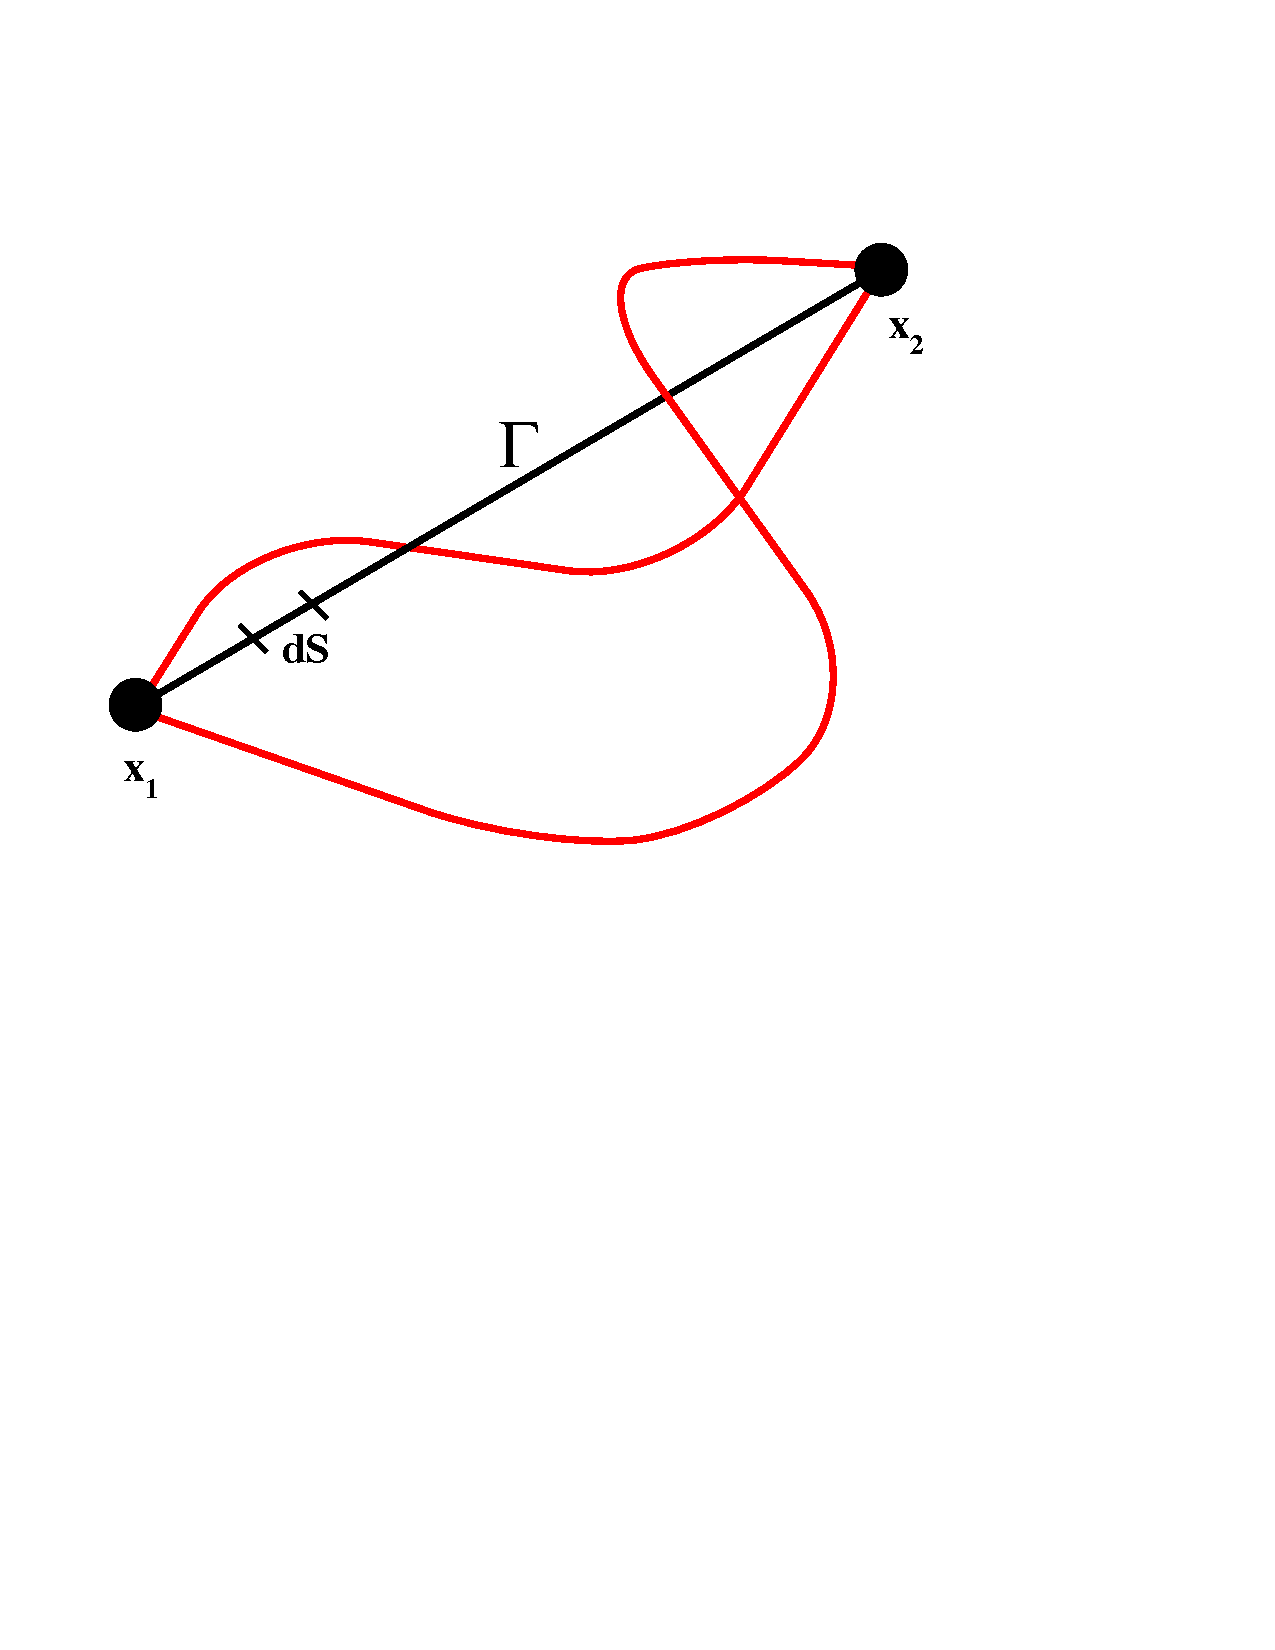
\includegraphics[width=0.66\linewidth]{Diagrams/varn_strt.pdf}
	 			\caption[]{What curve gives the shortest distance between two
	 			points in a plane ?  And how to prove it !}
	 			\label{fig:varn2}
	 		\end{center}
		\end{figure}
	
		We decide, arbitrarily, that we will make $x$ the independent variable
		and find a curve $y(x)$ which satisfies the minimum distance requirement.
		
		The distance along a curve is a path integral :
			\begin{equation}
				S = \int_{x_1}^{x_2} \frac{ds}{dx} dx	
			\end{equation}
		where
			\begin{equation}
				\frac{ds}{dx} = \sqrt{1 + \left( \frac{dy}{dx} \right)^2}
			\end{equation}
		We seek to find $y(x)$ which minimizes $S$. First consider the 
		function
			\begin{equation}
				\begin{split}
				Y(x,\alpha) &= y(x) + \alpha \eta(x) \\
				\frac{\partial Y}{\partial x} \equiv Y' &= y'(x) + \alpha \eta'(x)
				\end{split}
			\end{equation}
		where $\eta(x)$ is an arbitrary function which is differentiable and
		vanishes at $x=x_1,x_2$. This is the variation which we apply to
		some curve $y(x)$ to see if it gets shorter or longer. Note the notation
		for the derivative which will be useful as we procede.
	
		The optimal path will minimize	 $S(\alpha)$, when $\alpha=0$, i.e.
			\begin{equation}
				\left. \frac{\partial S(\alpha)}{\partial \alpha} \right|_{\alpha = 0} = 0
			\end{equation}
		In our current notation
			\begin{equation}
				S(\alpha) = \int_{x_1}^{x_2} \sqrt{1 + (Y')^2}
			\end{equation}
		and 
			\begin{equation}
				\frac{\partial S(\alpha)}{\partial \alpha} = 
					\int_{x_1}^{x_2}  \frac{1}{2} \frac{1}{\sqrt{1 + (Y')^2}} . 2 Y' \frac{\partial Y'}{\partial \alpha} dx
			\end{equation}
		from the definition of $Y'(x,\alpha)$
			\begin{equation}
				\frac{\partial Y'}{\partial \alpha} = \eta'(x)
			\end{equation}
	
		So we now must solve
			\begin{equation}
				\left. \frac{\partial S(\alpha)}{\partial \alpha} \right|_{\alpha = 0} =
					\int_{x_1}^{x_2} \frac{y'(x)\eta'(x)}{\sqrt{1 + (y')^2}} dx = 0
			\end{equation}
		We integrate by parts to give
			\begin{equation}
				\left. \frac{\partial S(\alpha)}{\partial \alpha} \right|_{\alpha = 0} =
					\left[   \frac{y'(x)\eta(x)}{\sqrt{1 + (y')^2}} \right]_{x_1}^{x_2} - 
					\int_{x_1}^{x_2} \eta{x} \frac{d}{dx} \frac{y'(x)}{\sqrt{1 + (y')^2}} dx = 0
			\end{equation}
		The first term on the RHS vanishes because $\eta$ vanishes at the boundaries. The
		second term is valid for arbitrary $\eta(x)$ which implies
			\begin{equation}	
				 \frac{d}{dx} \frac{y'(x)}{\sqrt{1 + (y')^2}} dx = 0
			\end{equation}
		which in turn implies $y'=$constant, i.e. the equation of
		a straight line. 
		
		The important things to note here are that an integral method can be used
		to solve a simple geometrical problem and that the method itself
		includes the boundary conditions as a natural consequence of the way
		it is set up.
		
		The variational method can be generalized to solve more important problems.
		In particular, instead of solving each problem as we have for the straight
		line / distance question above, we solve a generic problem whose solutions
		we can apply immediately.
		
		\subsection{Generalizing}
		
		The general form works like this. To find the 
		function $y(x)$ which produces a stationary value of 
		the functional 
			\begin{equation}
				J=\int_{x_1}^{x_2} F(x,y,y') dx
			\end{equation}
		we work through the same procedure as above, and use the same
		arguments concerning the arbitrary nature of the variation to obtain
			\begin{equation}
				\frac{d}{dx}\frac{\partial F}{\partial y'} - \frac{\partial F}{\partial y} = 0
			\end{equation}
		This is known as the Euler equation.	
		Hamilton's principle states that mechanical systems evolve such that 
		the integral 
			\begin{equation}
				J=\int_{t_1}^{t_2} L dt
			\end{equation}
		is stationary. Here $L$ is the Lagrangian of the system which is
		identified with a combination of  the work done on the system and the kinetic energy 
		of the system, e.g. potential energy - kinetic energy.
		
		Application of the Euler equation to each direction independently
		recovers Newton's law ($F=ma$). In complex geometries and
		with difficult boundary conditions, the variational form
		may be easier to solve than the differential or ``strong'' form.
		
		\Red{This shows us that there are equivalent integral
		representations for the standard mechanical equations we
		are accustomed to using --- variational or weak forms
		versus differential or strong forms}.
		
		
		Although this may seem complicated and of rather theoretical interest, 
		in fact it runs throughout finite element
		methods, and the concept must be familiar in order to follow how FEM
		works.  
		Advantages of using variational forms of the equations include 
		
		%% As a bulletted list ??
		
		The simplification of the construction of the governing
		equations in the sense that scalar quantities --- energies,
		potentials --- are considered in place of forces, displacements
		etc. There is also the possibility that such formulations can 
		be derived more-or-less automatically for previously unknown
		systems.
		
		Governing equations may be more directly accessible since
		``unimportant'' variables such as internal forces doing no
		net work do not appear in the variational form.
		
		When dealing with approximate solutions, the variational form
		often allows a broader range of trial functions than for the 
		standard differential form. This happens because some boundary
		conditions are implicit in the formulation and hence are not imposed
		on the trial functions themselves.
		
		
	
		\subsection{Example of Variational Forms for FEM}
	
		\Emerald{See Klaus-J\"{u}rgen Bathe for details}
	
		
		%% FIGURE: heated bar
			\begin{figure}[h]           
				\begin{center}
		 			 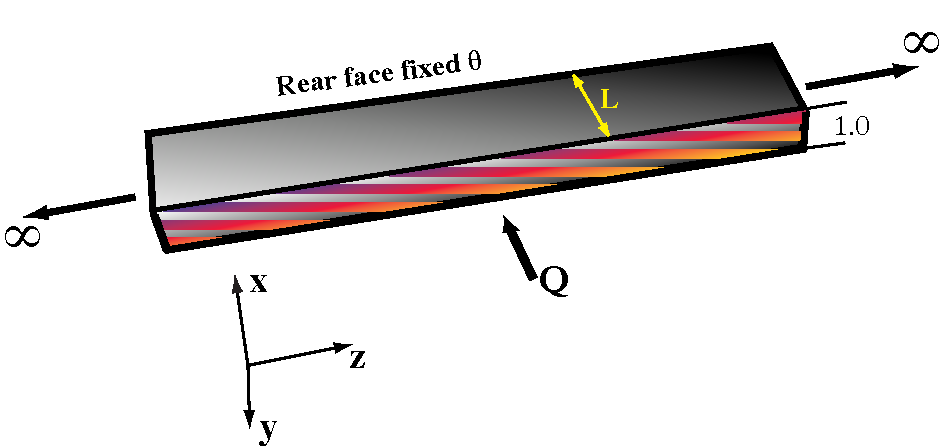
\includegraphics[width=0.66\linewidth]{Diagrams/heatcond.pdf}
		 			\caption[]{A Slab of Material Subjected to an sudden onset of heating at $Q$ on one side 
		 			at time $t=0$}
		 			\label{fig:heat1}
		 		\end{center}
			\end{figure}
	
		The functional governing the temperature in the slab of figure \ref{fig:heat1} is
			\begin{equation}
				\Pi = \int_0^L \frac{1}{2} k \left(\frac{\partial \theta}{\partial x} \right)^2 dx -  
								\int_0^L \theta q^B dx - \theta(0,t) Q
			\end{equation}
		where $q^B$ is an internal heat generation rate. The fixed boundary
		condition is $\theta(L,t) =\theta_i$.
		
		This is our generalized problem with 
			\begin{equation}
					F = \frac{1}{2}k  \left(\frac{\partial \theta}{\partial x} \right)^2 - \theta q^B
						= \frac{1}{2}k {\theta'}^2 - \theta q^B
			\end{equation}
		which produces a stationary functional if
			\begin{equation}
					\frac{d}{dx}\frac{\partial F}{\partial \theta'} - \frac{\partial F}{\partial \theta} = 0	
			\end{equation}
		or, in other words
			\begin{equation}
				k\frac{d^2 \theta}{d x^2} = q^B	
			\end{equation}
		Which we recognize to be the governing differential equation. The variational
		statement also contains the natural boundary condition
			\begin{equation}
				 k \left. \frac{\partial \theta}{\partial x}	\right|_{x=0} + Q = 0
			\end{equation}
			
		This is a clear demonstration that the standard form of the equations plus
		certain boundary conditions can be fully wrapped up in integral form and  
		are exactly equivalent to the standard form.
		
		The major difficulty is in how we produce the correct functional in 
		the first place, especially if we want to avoid first deriving 
		the differential form of the equations
		and back-calculating as we done above.
					
		\subsection{Extension to Approximate Methods}	
	
		The problem above is simple enough that the integral or differential forms
		of the equations can be solved directly. In general, however, we anticipate
		dealing with problems where no closed form of solution exists. Under these
		circumstances approximate solutions are desirable. In particular, there
		is a class of approximation methods which use families of trial functions
		to obtain a best fit approximation to the solution. These naturally
		develop into finite element algorithms as we shall soon see.
		
	\subsection{A Generic Problem Formulation}
		
	We consider a steady-state problem characterized by the following 
	strong form
		\begin{equation}
			{\cal{L}} (\phi) = f
		\end{equation}		
	where ${\cal{L}}$ is a linear differential operator acting on the 
	(unknown) state variable $\phi$ in responce to a forcing function $f$.
	Boundary conditions are
		\begin{equation}
			{\cal{B}}_i [\phi] = \left. q_i \right|_{\mbox{\small at boundary } S_i}    \mbox{\hspace{1cm}} i=1,2,\ldots
		\end{equation}

	The operator should be symmetric 
		\begin{equation}
			\int_\Omega v {\cal{L}}(u) d\Omega =  \int_\Omega u {\cal{L}}(v) d\Omega 
		\end{equation}
	 and positive definite
	 	\begin{equation}
	 		\int_\Omega u {\cal{L}}(u) d\Omega > 0
	 	\end{equation}
	 $\Omega$ is the domain of the operator and $u$ and $v$ are any functions
	 which satisfy the boundary conditions.	
	 
	 	%% FIGURE: stiff rod being pulled
			\begin{figure}[h]           
				\begin{center}
		 			 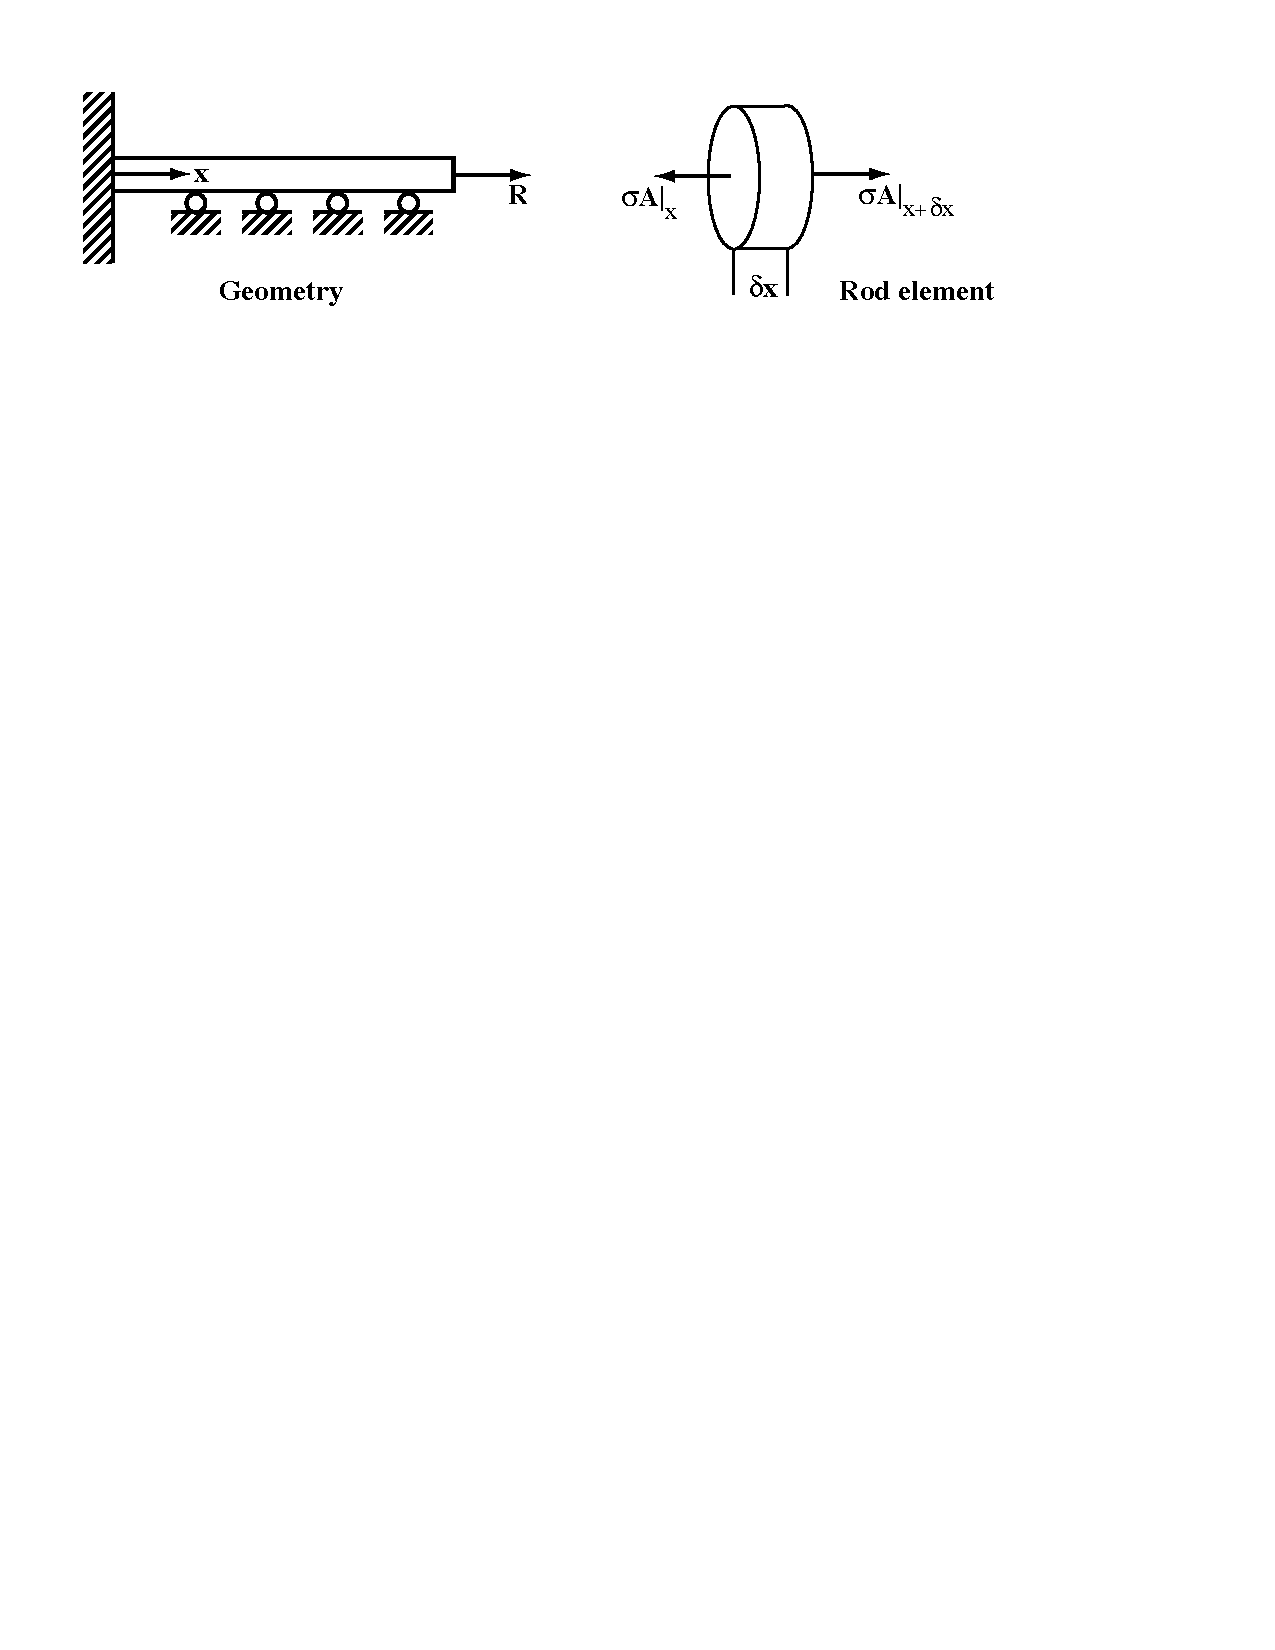
\includegraphics[width=0.66\linewidth]{Diagrams/rodpull.pdf}
		 			\caption[]{A rod subject to end load --- Young's modulus, $E$, density, $\rho$,
		 			cross sectional area, $A$}
		 			\label{fig:rod1}
		 		\end{center}
			\end{figure}
	 
	 Consider the 1D example of a bar subject to a steady end load. The
	 response is the solution to 
	 	\begin{equation}
	 		-EA\frac{\partial^2 u}{\partial x^2} = 0
	 	\end{equation} 
	 subject to the boundary conditions
	 	\begin{equation}
	 		\begin{split}
	 			\left. u \right|_{x=0} & = 0 \\
	 			\left. EA\frac{\partial u}{\partial x} \right|_{x=L} = R
	 		\end{split}
	 	\end{equation}
	 We therefore identify
	 	\begin{eqnarray*}
	 		{\cal{L}}= -EA\frac{\partial^2 u}{\partial x^2} & \phi = u & f = 0 \\
	 		& B_1 = 1 ; q_1 = 0 & \\
	 		& B_2 =  EA\frac{\partial }{\partial x}; q_2 = R & 
	 	\end{eqnarray*}
	 To check symmetry and positive definiteness of the operator we
	 consider $R=0$ since the operator properties are independent of the
	 actual load. Integrating by parts gives
	 	\begin{equation}
	 		\begin{split}
	 		\int_0^L-EA\frac{\partial^2 u}{\partial x^2} v dx & = 	
	 			- \left. EA\frac{\partial u}{\partial x} v \right|_0^L + \int_0^L EA \frac{\partial u}{\partial x} \frac{\partial v}{\partial x} dx \\
	 			 &= - \left. EA\frac{\partial u}{\partial x} v \right|_0^L  - \left. + EA u \frac{\partial v}{\partial x}  \right|_0^L
	 			 - \int_0^L EA\frac{\partial^2 v}{\partial x^2} u dx
	 		\end{split}	
	 	\end{equation}
	 Application of boundary conditions demonstrates that the operator is
	 symmetric by our definition.
	 
	 Positive definiteness is also assured since
		 \begin{equation}
		 		\int_0^L-EA\frac{\partial^2 u}{\partial x^2} u dx = 	
		 			- \left. EA\frac{\partial u}{\partial x} u \right|_0^L + \int_0^L EA \frac{\partial u}{\partial x} \frac{\partial u}{\partial x} dx 		=
		 			0 + \int_0^L EA \left(\frac{\partial u}{\partial x}\right)^2 dx 		
		 \end{equation}
	
	Suppose we now search for approximate solutions of the form
		\begin{equation}
			\bar{\phi} = \sum_{i=1}^{n} a_i \Phi_i	
		\end{equation}
	where $\Phi_i$ are linearly independent trial functions and the $a_i$ are
	the unknown weights for each of the functions.
	
	In weighted residuals methods, the expansion is used directly
	on the strong form of the equations. $\Phi_i$ are chosen so
	as to satisfy all boundary conditions and then we seek to 
	minimize a residual
		\begin{equation}
			R = f - {\cal{L}}( \sum_{i=1}^{n} a_i \Phi_i	)
		\end{equation}		
		 	
	\subsubsection{Least Squares Method}	 	
	 Minimize the square of the residual with respect to $a_i$
	 	\begin{equation}
	 		\frac{\partial}{\partial a_i} \int_\Omega R^2 d\Omega = 0   \mbox{\hspace{1cm}} i = 1,2,\ldots
	 	\end{equation}
	 This method produces a symmetric coefficient matrix regardless of the
	 properties of the operator.	
	 	
	\subsubsection{Galerkin Method}
	To determine $a_i$, solve the n equation system
		\begin{equation}
			\int_\Omega N_i R d\Omega = 0	 \mbox{\hspace{1cm}} i = 1,2,\ldots
		\end{equation}		
	over the solution domain $\Omega$. This method produces a 
	symmetric, positive definite coefficient matrix if the operator is 
	symmetric and positive definite.
		 	
	\subsubsection{Ritz Method}	 	
	The Ritz method does not operate on the residual of the strong problem,
	but minimizes the weak form of the problem with respect to each of the
	unknown parameters $a_i$ in the usual variational manner. The trial 
	functions no longer need satisfy the natural boundary conditions
	of the problem as these are wrapped up in the variational form.
	\Emerald{(Again, see Bathe for discussion and examples).	 	}
		 	
	The Galerkin method can be extended to include a term which 
	minimizes the violation of natural boundary conditions, and thus
	permits the use of a wider range of trial functions	 	
		 \begin{equation}
			\int_\Omega N_i R d\Omega  + \int_\Gamma N_i R_B d\Gamma = 0	 \mbox{\hspace{1cm}} i = 1,2,\ldots
			\label{eq:galerk1}
		\end{equation}		
	However, it does not now necessarily produce a symmetric matrix even
	for a symmetric operator. However, if the equation (\ref{eq:galerk1} ) is
	integrated once by parts, it yields a symmetric form and also reduces
	the order of derivatives inside the integral. This means that 
	the trial functions need be of lower order, and it makes the
	Galerkin formulation equivalent to the Ritz formulation.
		
	Weighted residual formulations have one advantage: they can be used
	whether or not there exists a functional corresponding
	to the particular problem.	As a result is used this method is used extensively in 
	constructing finite element methods.		
		
	\section{Finite Element Theory}
	
	\subsection{The Genesis of a Matrix Method}
			
		One of the dominant features of the Finite Element literature
		is that it is filled with matrix algebra. The fact that differential
		equations can be rendered into matrices seems at first to be
		mysterious. However, it results quite naturally from the 
		discretization of the problem, and the parameterization of the
		discrete equations through a limited set of unknown parameters.
		
		Thus, before getting deeply involved in the arcane lore of Finite Elements,
		We give one example of a genuinely discrete system and show
		how it generates a matrix problem quite naturally. 
			
			
		%% FIGURE: stiff rod being pulled (don't look that up on the internet)
			\begin{figure}[h]           
				\begin{center}
		 			 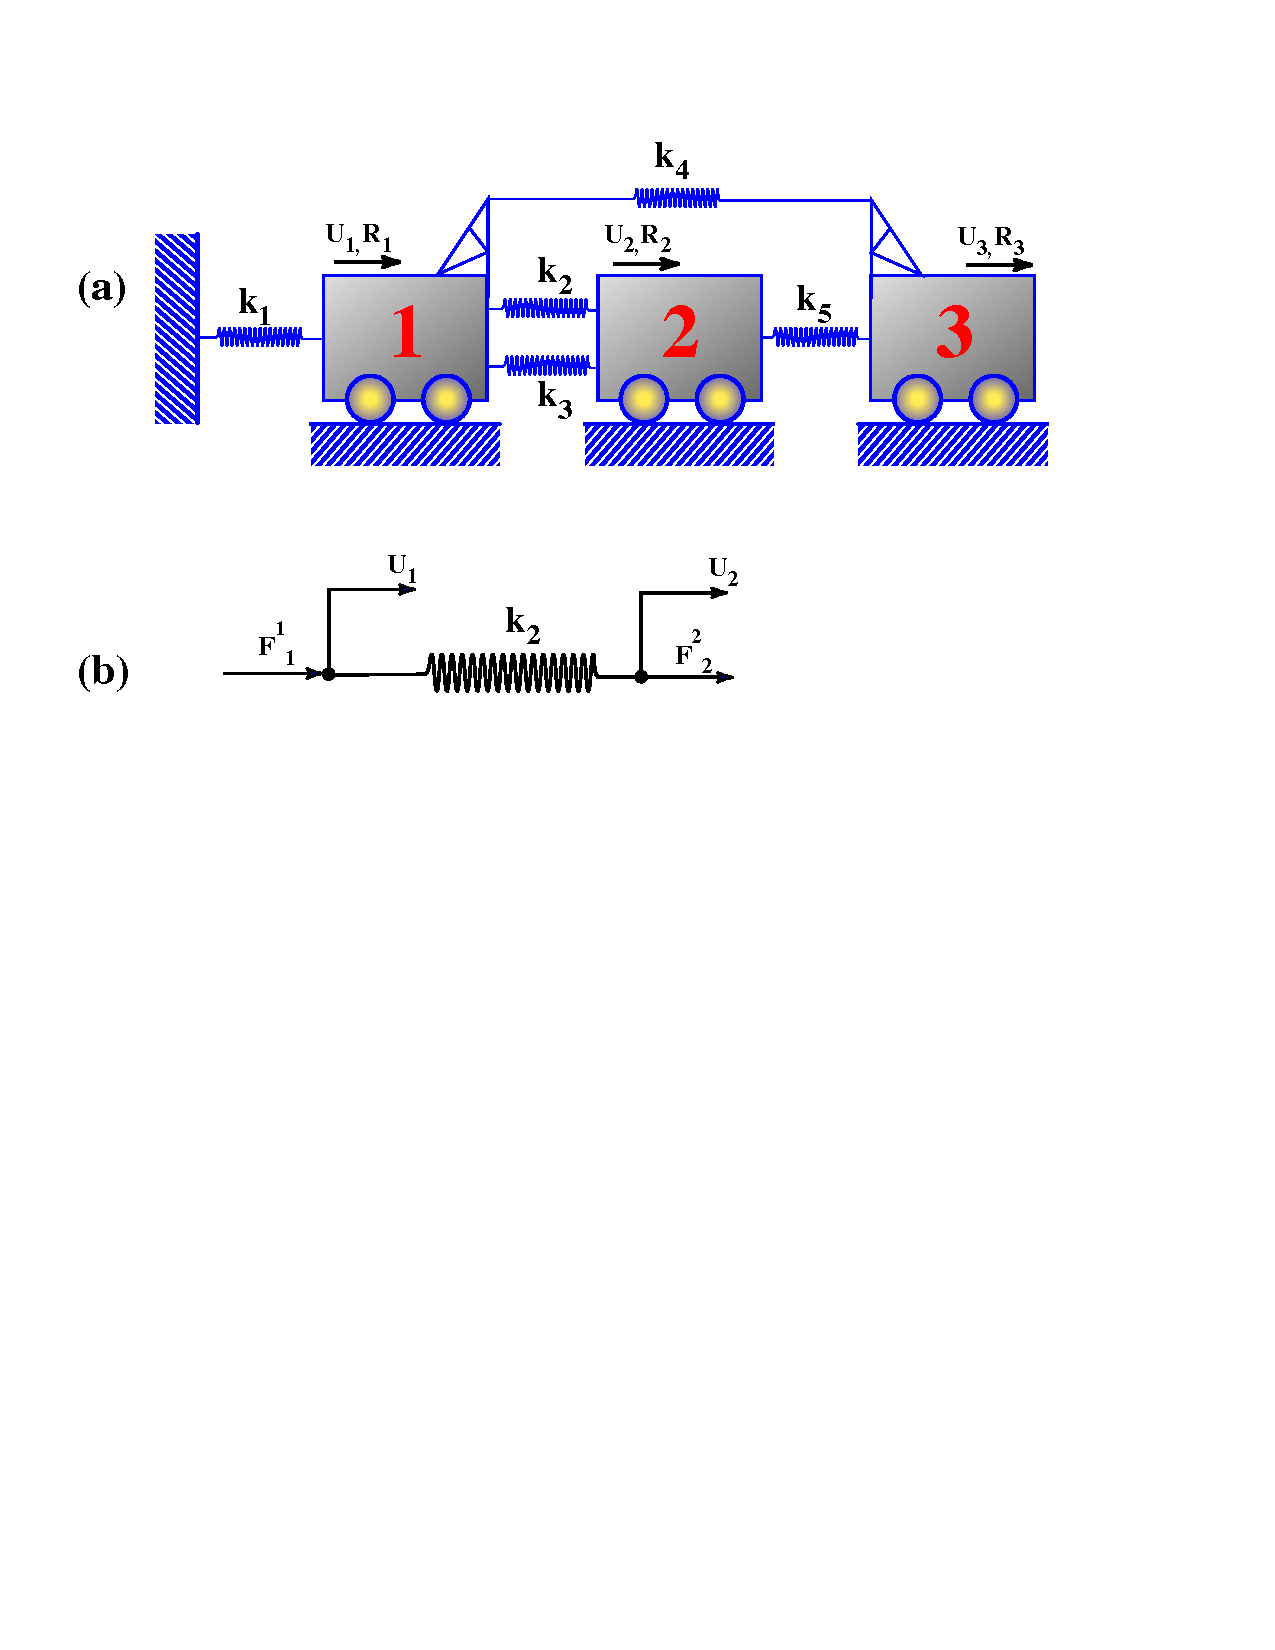
\includegraphics[width=0.66\linewidth]{Diagrams/carts.pdf}
		 			\caption[]{(a) A system of three carts interconnected by springs of different stiffnesses and
		 			in turn connected to an end wall. (b) The element equilibrium diagram for the spring $k_2$}
		 			\label{fig:cart1}
		 		\end{center}
			\end{figure}	
			
	Consider the system illustrated in Figure \ref{fig:cart1}a --- three freely rolling carts
	attached by springs. There are three loads applied $R_1,R_2,R_3$, one to each cart, and we wish 
	to determine the equilibrium displacements $U_1,U_2,U_3$.  In Figure \ref{fig:cart1}b we
	illustrate the equilibrium condition for one of the springs based on its internal degrees
	of freedom and effective external load. This equilibrium is:
			\begin{equation}
					\begin{split}
							k_2 (U_1 - U_2) &= {F_1}^{(2)} \\
							k_2 (U_2 - U_1) &= {F_2}^{(2)}
					\end{split}
			\end{equation}
	or
			\begin{equation}
					k_2	\left[  \begin{array}{cc}  1 & -1 \\ -1 & 1 \end{array} \right]
							\left[		\begin{array}{c} U_1 \\ U_2 \end{array} \right] = 
							\left[		\begin{array}{c} {F_1}^{(2)} \\ {F_2}^{(2)}\end{array} \right] 
			\end{equation}
	 This is essentially the same for all five spring elements
	 except for $k_1$ which is anchored at one end and
	 so satisfies
	 	\begin{equation}
	 		k_1 U_1 = {F_1}^{(1)}
	 	\end{equation}
		 
	 The equilibrium relations for the system as a whole are 
	 		\begin{equation}
					\begin{split}
						& {F_1}^{(1)} + 			{F_1}^{(2)} + 			{F_1}^{(3)} + 			{F_1}^{(4)} = R_1 \\
						& {F_2}^{(2)} + 			{F_2}^{(3)} + 			{F_2}^{(5)} = R_2 \\
						& {F_3}^{(4)} + 			{F_3}^{(5)} = R_3
					\end{split}
					\label{eq:globeq}
			\end{equation}
		
	If we now write all five equilibrium relations in terms of all available degrees of 
	freedom we obtain a form like this
		\begin{equation}
				k_2	\left[  \begin{array}{ccc}  k_2 & -k_2 & 0  \\ -k_2 & k_2 & 0 \\ 0 & 0 & 0 \end{array} \right]
						\left[		\begin{array}{c} U_1 \\ U_2 \\ U_3 \end{array} \right] = 
						\left[		\begin{array}{c} {F_1}^{(2)} \\ {F_2}^{(2)} \\ 0\end{array} \right] 
		\end{equation}
	which can also be written
		\begin{equation}
			\mathbf{K}^{(2)}\mathbf{U} = \mathbf{F}^{(2)}
		\end{equation}
	in each case.
	
	Thus the global equilibrium requirement of \ref{eq:globeq} become
		\begin{equation}
			\mathbf{K}\mathbf{U} = \mathbf{R}
		\end{equation}
	where
		\begin{equation}
			\mathbf{K} = \left[
			\begin{array}{ccc}
				(k_1 + k_2 +k_3 + k_4) & -(k_2+k_3) & -k_4 \\
				-(k_2+k_3) & (k_2 + k_3+k_4) & -k_5 \\
				-k_4 & -k_5 & (k_4 + k_5)
			\end{array}
			\right]
		\end{equation}	
	Note, by the way, that $ \mathbf{K}$ is symmetric.
	An important observation is that 
		\begin{equation}
			\mathbf{K} = \sum_{i=1}^{5} \mathbf{K}^{(i)}
		\end{equation}
	The individual element stiffnesses can be summed to form a
	global stiffness matrix. A symmetric, positive definite
	matrix problem can be solved in numerous different ways, many
	of which are easy to look up in textbooks !

	A very simple problem like this has captured much of what
	we need to do in arbitrarily complex finite element computations.
	The construction of local element equilbrium problems based
	on the interaction of each available degree of freedom with
	every other is followed by the assembly into a 
	global problem by summing the contributions of the individual 
	elements.
	
	Note that the formulation of the local equilibrium conditions
	are done in a symmetric manner (if we change this degree of 
	freedom how does the balance change, and then what if we change
	this degree of freedom ?) rather than trying to simplify the system.
	
	The degrees of freedom are related by elastic spring constants 
	here. In our more abstract formulations we will replace spring 
	constants by coefficients obtained from the variational method but
	the form is {\em exactly the same}.  
	

	\subsection{Weak Forms of Real Equations}
		
	As we discovered earlier, the Galerkin form of weighted residual approximate
	method can be made equivalent to a full variational problem if
	integration by parts is employed in the correct manner. This then
	allows the development of fully automatic variational methods
	for arbitrary strong forms of the governing equations. From here
	on we follow the notation of Hughes (The Finite Element Method)
	which is reasonably clear and also coincides with the internal
	nomenclature of CITCOM.
	
	\subsubsection{1D Heat Conduction}
	
	The differential or strong form of the equation we have encountered
	a number of times is 
		\begin{equation}
			\begin{split}
				\frac{d^2 u}{d x^2} - {\curly f} &= 0  \mbox{\hspace{1cm} on $\Omega$} \\
				u(1) & = {\curly g} \\
				-\frac{d u}{d x} (0) &= {\curly h}
			\end{split}
		\end{equation}
	where the boundary conditions are supplied at either end of a domain
	of unit length.
	
	To find the weak form of the equation we need to have a set of 
	functions $\curly S$ to use for the trial functions which satisfy the boundary
	condition $\curly g$ on $u$ at $x=1$. We also need a set of weighting
	functions which are zero at $x=1$ which we call $\curly V$. The weighting
	functions play the role of the variations.
	
	The statement of the weak form of the problem (as distinct from
	its solution which will wait till later) is then to find $u \in {\curly S}$ such 
	that for all $w \in {\curly V}$
		\begin{equation}
			\Red{ \int_0^1 \frac{d w }{d x} \frac{d u}{d x} dx - \int_0^1 w f dx + w(0) h = 0 }
		\end{equation}
	
	This looks a lot like the variational solutions we found before. How do we get to it ?
	The procedure is relatively general (except that in higher dimensions it becomes more 
	time consuming). First assume we have found the solution to the strong form, $u$. This must
	satisfy
		\begin{equation}
			0 = \int_0^1 w( \frac{d^2 u}{d x^2} - {\curly f} )dx
		\end{equation}
	by the definition of the problem, as long as $w$ is well behaved, which 
	is ensured by a sensible choice of weighting functions. This starts to look
	a lot like the Galerkin approach although we are not yet seeking an approximate
	solution. Now integrate by parts to give 
		\begin{equation}
			0 = \int_0^1 \frac{d w }{d x} \frac{d u}{d x} dx - \int_0^1 w f dx - \left[ w \frac{d u}{d x} \right]_0^1
		\end{equation}
	the boundary conditions on $du / dx$ are substituted to give the weak form as above.
	We write the equation in terms of the symmetric operators:
		\begin{equation}
			\begin{split}
			a(w,u) & \equiv 	\int_0^1 \frac{d w }{d x} \frac{d u}{d x} dx \\
			(w,{\curly f})  & \equiv  \int_0^1 w f dx
			\end{split}
		\end{equation}
	to obtain an abstract form which can be used for all the finite element
	formulations we derive here
		\begin{equation}
			a(w,u) = (w,{\curly f})  + w(0){\curly h}
			\label{eq:FEabst}
		\end{equation}
	
	
	Note, that the partial differentiation step produces a symmetric operator from the
	non symmetric initial form. This approach also works in 2D as follows.	
	
	\subsubsection{2D Heat Conduction}
	Define a heat flux (vector), $\mathbf{q}$ related to temperature, $u$ as 	follows
		\begin{equation}
			q_i = -K_{ij} \frac{\partial u}{\partial x_j}
		\end{equation}
	where $mathbf{K}$ is the symmetric conductivity tensor. (This is 
	the generalized version of Fourier's law). A volumetric heating rate of $\curly f$ 
	gives the following strong form
		\begin{equation}
			\begin{split}
				\nabla q - {\curly f} &= 0  \mbox{\hspace{1cm} on $\Omega$} \\
				u & = {\curly g} \mbox{\hspace{1cm} on $\Gamma_{\curly g}$} \\
				-q_i n_i &= {\curly h} \mbox{\hspace{1cm} on $\Gamma_{\curly h}$}
			\end{split}
		\end{equation}
	where $\Gamma_ {\curly g}$ and $\Gamma_{\curly h}$ are the regions of the boundary
	with fixed temperatures and fixed fluxes respectively, $\mathbf{n}$ is the unit normal
	over $\Gamma_{\curly h}$.
	
	The corresponding weak form (found in the usual way) is 
		\begin{equation}
			-\int_\Omega  \frac{\partial w}{\partial x_j} q_i d\Omega = \int_\Omega w {\curly f} d\Omega + \int_{\Gamma_{\curly h}} w{\curly h} d\Gamma
		\end{equation}
	The symmetry of the operator is not obvious here until we substitute the constitutive law to obtain
		\begin{equation}
			\int_\Omega  \frac{\partial w}{\partial x_j} q_i d\Omega =
			 \int_\Omega  \frac{\partial w}{\partial x_j} K_{ij} \frac{\partial u}{\partial x_j} d\Omega = 
			 \int_\Omega  (\nabla w)^T \mathbf{K} (\nabla u) d\Omega
		\end{equation}
		
	\subsubsection{2D/3D Fluid Flow}
	Now we finally come around to the problem we really need to solve.
	The strong form of the Stokes' flow problem is identical to that
	of linear elasticity (which is what all the finite element textbooks
	deal with).
	
	The general constitutive law is
		\begin{equation} 
			\sigma_{ij} = c_{ijkl} \epsilon_{kl}
		\end{equation}
	which reduces to $\sigma_{ij} = \eta \epsilon_{ij}$ for homogeneous fluid.
	$\epsilon_{ij}$ is defined by
		\begin{equation}
			\epsilon_{ij} = \frac{\partial u_i}{\partial x_j} +  \frac{\partial u_j}{\partial x_i}
		\end{equation}
	where $\mathbf{u}$ now represents the fluid velocity.
	
	The strong form of the equation is
		\begin{equation}
			\begin{split}
				\frac{\partial \sigma_{ij}}{\partial x_j} + {\curly f}_i = 0  \mbox{\hspace{1cm} on $\Omega$} \\
					u_i & = {\curly g}_i \mbox{\hspace{1cm} on $\Gamma_{{\curly g}_i}$} \\
				 	\sigma_{ij} n_i &= {\curly h}_i \mbox{\hspace{1cm} on $\Gamma_{{\curly h}_i}$}
			\end{split}
		\end{equation}
	with a corresponding weak form
		\begin{equation}
			\int_\Omega \left(  \frac{\partial w_i}{\partial x_j} +  \frac{\partial w_j}{\partial x_i}  \right) \sigma_{ij} d \Omega =
				\int_\Omega w_i {\curly f}_i d\Omega + 
				\sum_{d=1}^{n_{\rm dim}} \left[ \int_{\Gamma_{{\curly h}_i}} w_i h_i d\Gamma \right]
		\end{equation}
	Which is symmetric in the trial functions and the unknown velocities since
		\begin{equation}
			\int_\Omega \left(  \frac{\partial w_i}{\partial x_j} +  \frac{\partial w_j}{\partial x_i}  \right) \sigma_{ij} d \Omega =
			\int_\Omega \left(  \frac{\partial w_i}{\partial x_j} +  \frac{\partial w_j}{\partial x_i}  \right) c_{ijkl}
				\left(  \frac{\partial u_i}{\partial x_j} +  \frac{\partial u_j}{\partial x_i} \right) d \Omega
		\end{equation}
	
	\subsection{Galerkin Approximate Weak Form}
	
	We have one last task before we can develop a real numerical method. How do 
	we get away from the highly abstract notion of trial functions, weighting functions, 
	and weak forms to produce a compact system of equations which 
	can be written out in a nice tidy matrix form.
	
	The answer lies in the Galerkin approximate solution method.
	Let us go back to the 1D problem for a moment.
	We have to express our solution in terms of a sum over basis functions as before
		\begin{equation}
				w^h = \sum_{A=1}^{n} c_A  N_A
		\end{equation}
	where the $h$ superscript indicates that we have moved from an infinite choice of
	functions to a finite one based on the discrete functions $N_A$ which we will define
	in a minute, although for now we need to ensure that they are zero where the boundary conditions apply
	in the same way as $\curly V$. We define a corresponding expansion for $u$
		\begin{equation}
			\begin{split}
				u^h &= \sum_{A=1}^{n} d_A  N_A + {\curly g}N_{n+1} \\
				{\curly g}^h &= {\curly g} N_{n+1}
			\end{split}
		\end{equation}	
	which includes an extra basis function to allow the boundary condition ($u(1)={\curly g}$) to be satisfied.
	
	Substituting into (\ref{eq:FEabst}) gives 
		\begin{equation}
			a\left( \sum_{A=1}^n c_A N_A , \sum_{B=1}^n d_B N_B \right) = 
			\left( \sum_{A=1}^n c_A N_A , {\curly f} \right) + \left[ \sum_{A=1}^n c_A N_A(0) \right] {\curly h}
			-a\left( \sum_{A=1}^n c_A N_A , {\curly g} N_{n+1} \right)
		\end{equation}
	Our operators are symmetric and wholly linear, so the order of summation and application
	of the operator can be interchanged freely to give:
		\begin{equation}
			0 = 	\sum_{A=1}^n c_A G_A
		\end{equation}
	where
		\begin{equation}
			G_A = \sum_{B=1}^n a(N_A,N_B)d_B - (N_A,{\curly f}) - N_A(0){\curly h} + a(N_A,A_{n+1}){\curly g}
		\end{equation}
	As so often before, resort the argument that the particular choice of variation must 
	be totally arbitrary: this equation must hold no matter what $w^h \in {\curly S}^h$ we choose, and
	hence no matter what the combination of $c_A$ may be.
	This then means that $G_A$ must be identically zero independent of $c_A$, i.e.
		\begin{equation}
			 \sum_{B=1}^n a(N_A,N_B)d_B =  (N_A,{\curly f} ) 
			 - N_A(0){\curly h} +
			  a(N_A,A_{n+1}) {\curly g}
			 \label{eq:gal2}
		\end{equation}
	
	As in the standard variational method, we have eliminated all
	references to the actual variation and left unknowns which only
	related to the physical variables (i.e. the coefficients of the expansion
	for $u$).
	
	If we simply write
		\begin{equation}
			\begin{split}
				K_{AB} &= a(N_A,N_B)\\
				F_A &= (N_A,{\curly f}) + N_A(0)h - a(N_A,N_n+1){\curly g}
			\end{split}
			\label{eq:FEstdform}
		\end{equation}
	then we have a matrix formulation immediately since (\ref{eq:gal2}) now becomes
		\begin{equation}
			\sum_{B=1}^n  K_{AB} d_B = F_A  \makebox[1cm]{} A=1,2,3,\ldots
		\end{equation}
	or 
		\begin{equation}
			\mathbf{K d} = \mathbf{F}
		\end{equation}
	The matrix $\mathbf{K}$ is known as the stiffness matrix --- the 
	association with the matrix of stiffnesses from our discrete set of springs
	being obvious.
		
	\subsection{Generalization}
	
	The same argument can be applied to higher dimensions, and to problems
	with different constitutive laws, and 
	vector unknowns, however, the identification of the 
	components of the stiffness matrix with the operator $a(\cdot,\cdot)$ acting on
	every possible combination of the galerkin basis functions still holds.
	
	When the unknowns are vectors, the basis functions are used in each respective
	direction which complicates the notation even more than before. Essentially, though
	it means that the entries to $\mathbf{K}$ from each $A$ and $B$ are actually
	matrices which are $n_{\rm dim} \times n_{\rm dim}$.
	
	For example, in the constant viscosity Stokes' flow problem, we now have
		\begin{equation}
			\left. K_{AB}\right|_{ij}  = 	\int_\Omega
							\left(  \frac{\partial N_A}{\partial x_j} +  \frac{\partial N_A}{\partial x_i}  \right) \eta
							\left(  \frac{\partial N_B}{\partial x_j} +  \frac{\partial N_B}{\partial x_i} \right) d \Omega
				\label{eq:festokes}			
		\end{equation}
		
	\subsection{Discretization \& Shape Functions}
			
		Although we have now nominally made our problem finite by 
		expressing everything in terms of Galerkin basis functions, we have
		yet to decide what those functions ought to be. 
		Whatever our choice, it should make the problem easy to 
		compute numerically.
		
		 %% FIGURE: domain decomposition
			\begin{figure}[h]           
				\begin{center}
		 			 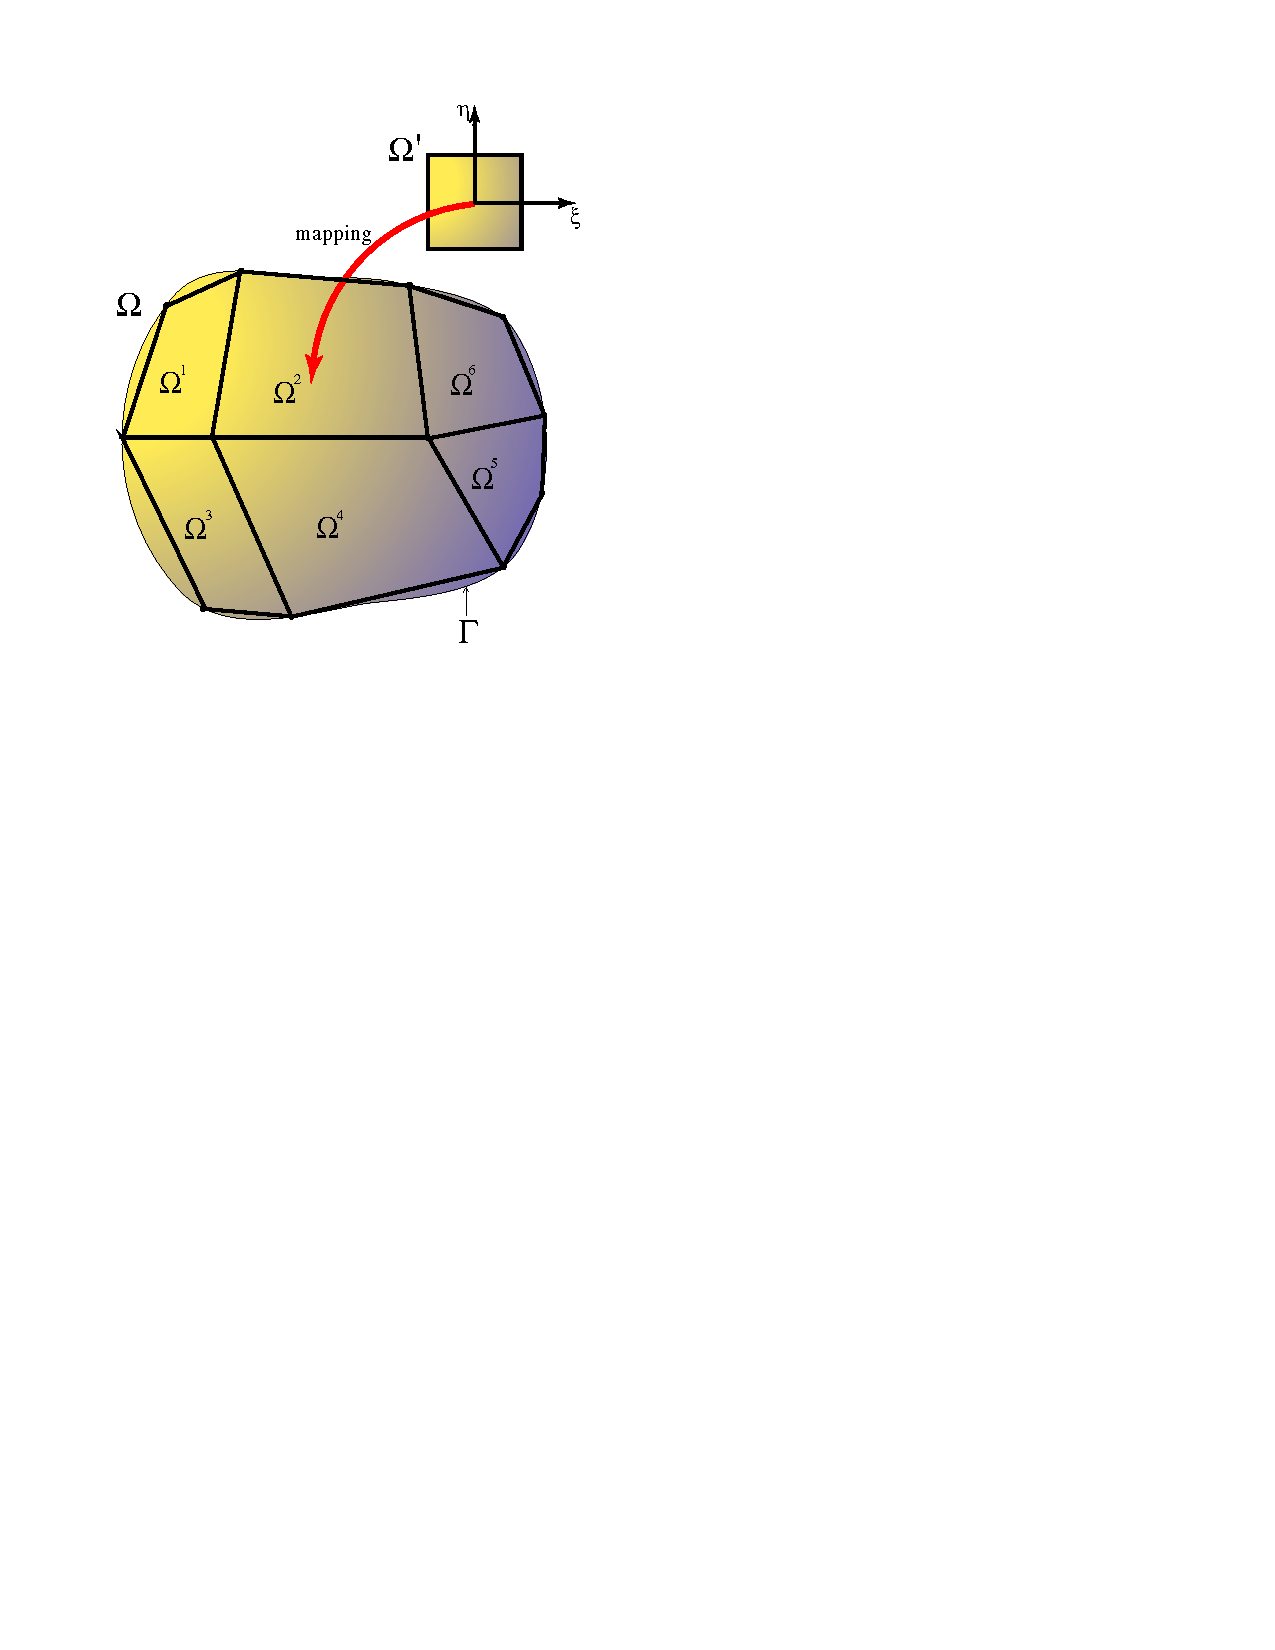
\includegraphics[width=0.66\linewidth]{Diagrams/domain.pdf}
		 			\caption[]{Splitting an arbitrary domain into patches is trivial in an 
		 			integral formulation. Additionally, the irregular shape of the 
		 			individual subdomains is easy to handle with standard 
		 			changes of variables (Jacobians)}
		 			\label{fig:domain}
		 		\end{center}
			\end{figure}	
		
		The choice of basis functions is very broad but we narrow it down 
		by tying it very closely to the way we choose to split up the domain of our problem.
		With an integral method, the domain decomposition is simple since
			\begin{equation}
					\int_\Omega d\Omega = \int_{\Omega_1} d {\Omega_1} + \int_{\Omega_2} d {\Omega_2} + \int_{\Omega_3} d {\Omega_3} + \ldots
					\label{eq:decomp}
			\end{equation}
		which means that the decomposition in Figure \ref{fig:domain} is as accurate as the representation of 
		the boundary allows.  
		
		The functions which interpolate the
		node points at the corners of  subdomains are a suitable set for
		use as an approximate basis as we require for the Galerkin
		formulation. This is easy to see if we consider a one dimensional
		problem.
		
				 %% FIGURE: domain decomposition
			\begin{figure}[h]           
				\begin{center}
		 			 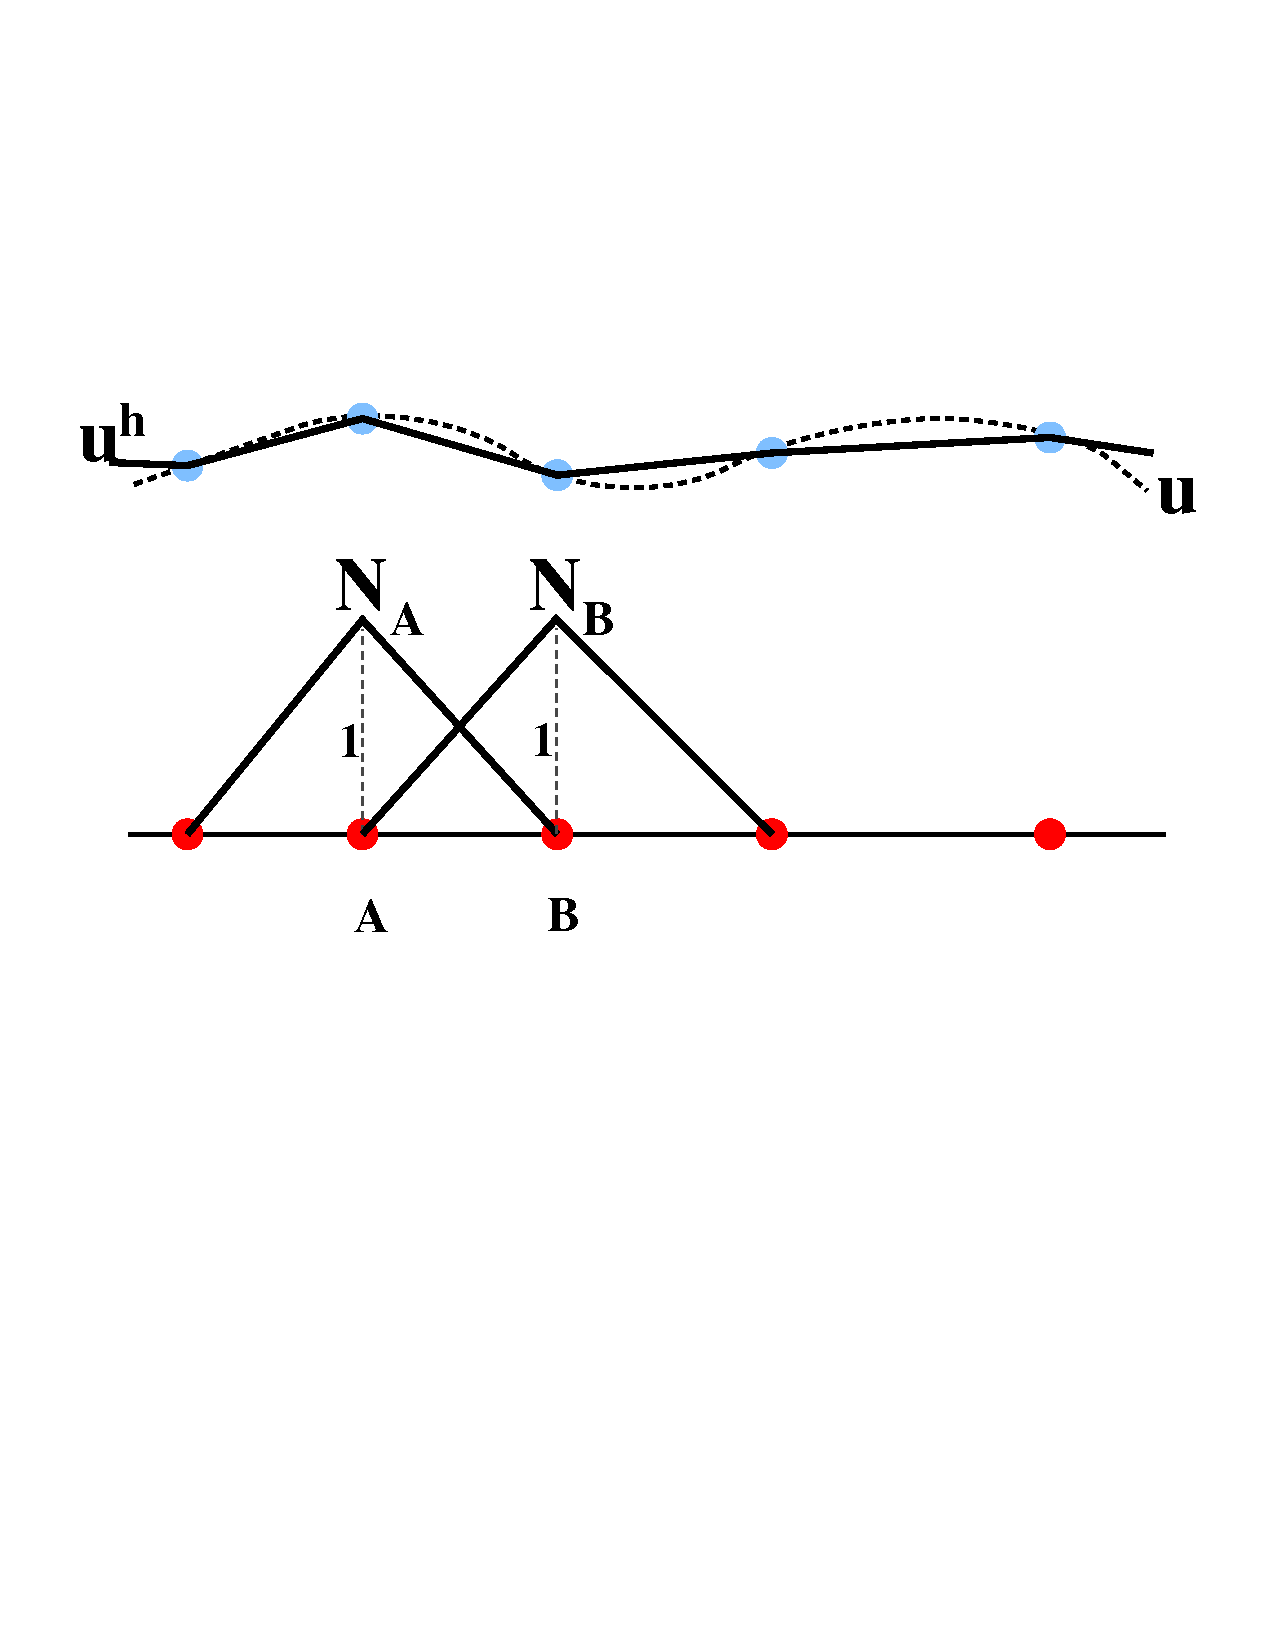
\includegraphics[width=0.66\linewidth]{Diagrams/linedisc.pdf}
		 			\caption[]{Representing a piecewise linear function as a sum
		 			of pointy functions localized at the nodes.}
		 			\label{fig:domain2}
		 		\end{center}
			\end{figure}	
	
		In the one dimensional case, the choice of subdomains is limited to breaking
		up the line into a number of segments, though not necessarily of equal
		length.	If the approximation to the continuum field, $u$ is made
		by linear interpolation to give $u^h$, then $u^h$ can also be
		expressed as a sum on the local triangular functions $N_A$ 
		as in Figure \ref{fig:domain2}
			\begin{equation}
				u^h = \sum_{A} u(x_A) N_A(x)
			\end{equation} 
		This is an exact representation of the interpolation provided
		the $N_A$ takes the value one at node $A$ and zero at
		all other nodes, and varies in a linear manner in between.
		
		 Note that the functions all take the 
		same form apart from scaling. Also, because the
		basis functions are localized around a node and its neighbours, 
		the direct interaction between a node and its immediate neighbours
		is non-zero but the interaction with more distant nodes is zero. This
		makes the stiffness matrix banded --- more importantly it is 
		sparse and therefore the potentially enormous number of interactions
		(the square of the number of unknowns) is contained.
		
		This procedure can be extended to higher dimensions and to 
		higher order interpolations as shown in Figure \ref{fig:sfn1}. 
		
		\subsubsection{Naming of Things and What They are Like}
		
		The interpolation functions are
		known as shape functions. 
		The subdomains are known as elements.
		The elements correspond to the individual springs of our
		discrete example.
		The shape functions are pure interpolation
		functions of the required order within the element and
		can be differentiated the appropriate number of 
		times. This means that the order of interpolation
		must match the order of derivatives in the FE operator.
		Crossing the element boundaries, the
		shape functions have discontinuous derivatives (as do the
		piecewise interpolations). Continuous derivative functions are
		possible (e.g. splines) but add significant complexity.
			Shape functions in 2D and 3D can be formed from the 
		product of 1D shape functions in each direction.
	
		 %% FIGURE: shape functions
			\begin{figure}[h]           
				\begin{center}
		 			 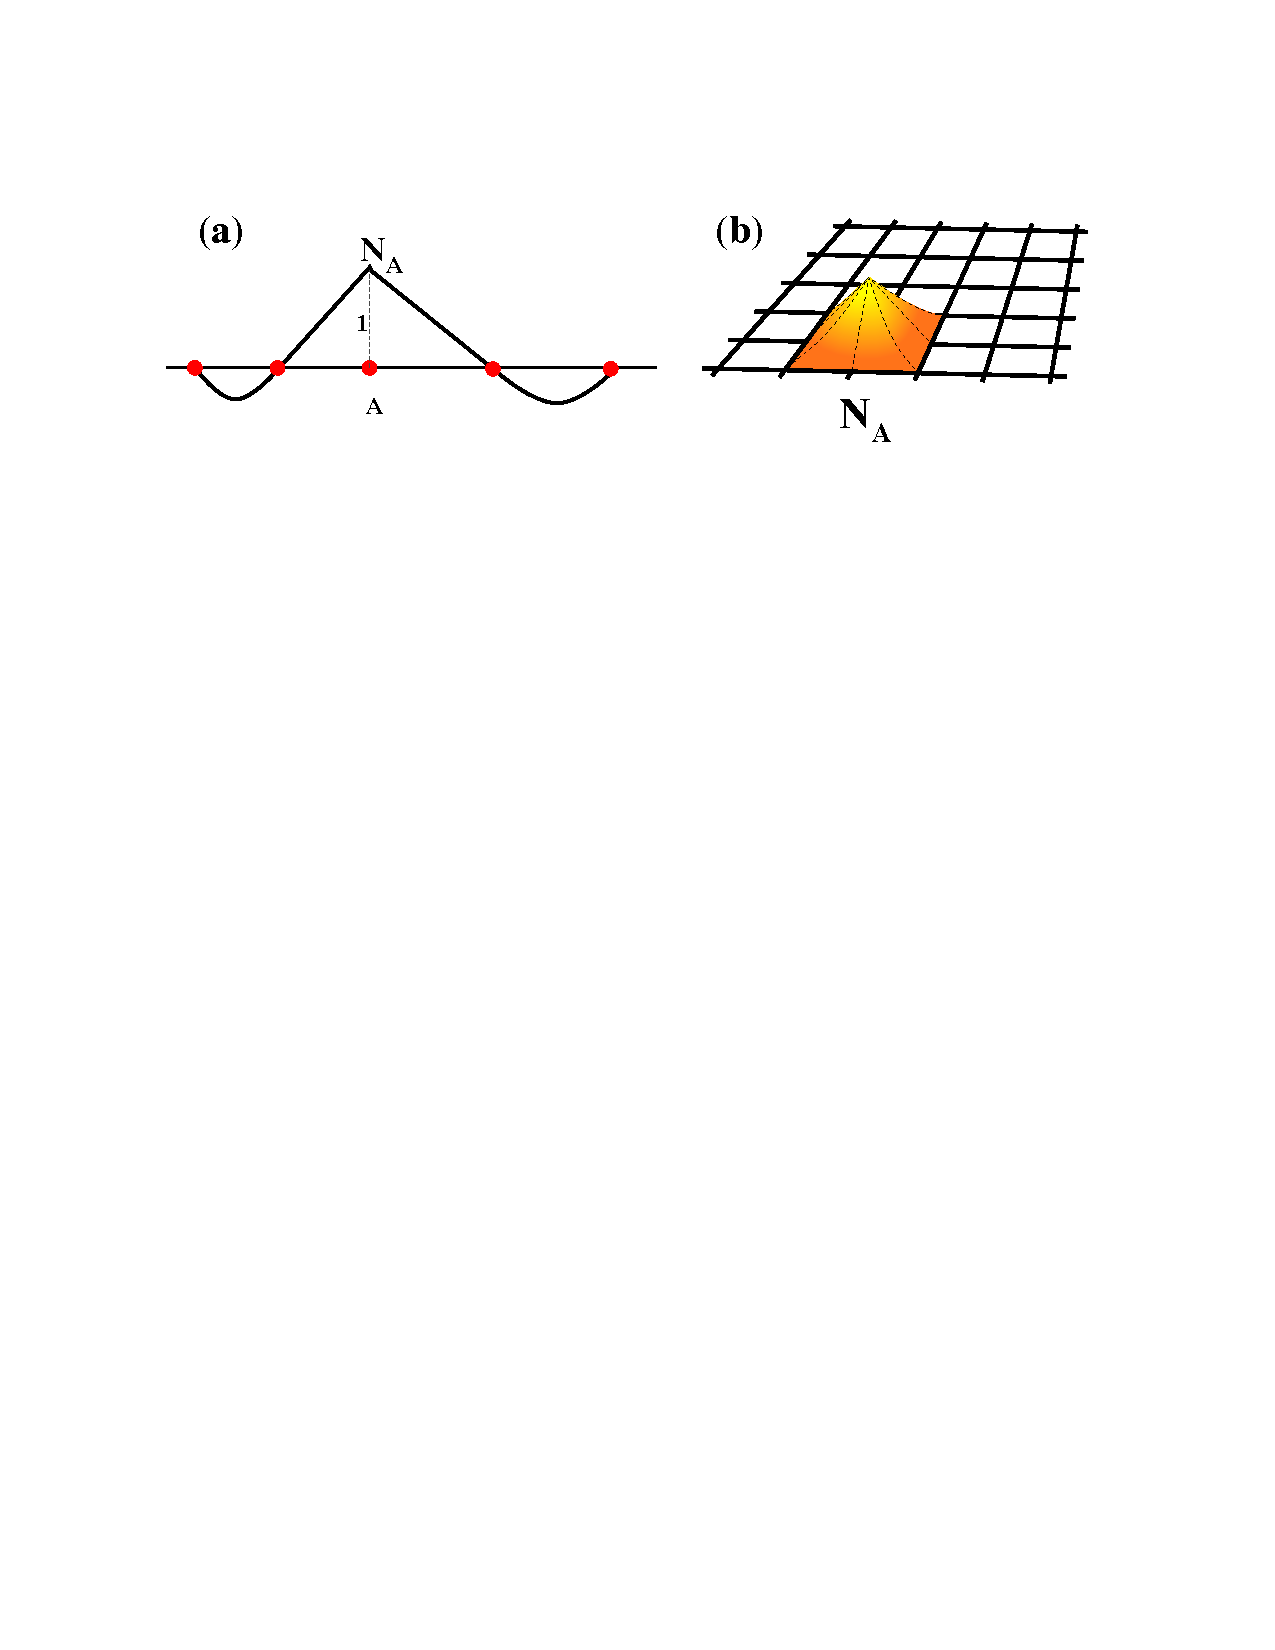
\includegraphics[width=0.66\linewidth]{Diagrams/shapefn.pdf}
		 			\caption[]{Extension of simple shape function concept (a) to 
		 			higher order functions and  (b) to higher dimensions}
		 			\label{fig:sfn1}
		 		\end{center}
			\end{figure}	
	
	\subsubsection{Element Matrices}
		
		The domain decomposition of (\ref{eq:decomp}) produces 
		a minature version of the matrix problem on the individual
		elements themselves.
			\begin{equation}
					{k^e}_{ij} {d^e}_j = {f^e}_i
			\end{equation}
		The interpretation of the local problem is similar to 
		that of the individual springs in the discrete example 
		we derived earlier. By assembling the 
		individual under-constrained element problems into the
		full problem we obtain a soluble system with the 
		correct number of boundary conditions etc.
	
		The local equilibrium problem is identical with 
		that of the global problem. That is, we use the
		same variational form and the same operators to 
		build the local matrices. In general, finite element
		methods are designed around the local element frame
		of reference and large problems assembled from 
		smaller ones. The book-keeping involved is to 
		track which degrees of freedom in the local 
		problem are associated with which others
		in the global problem. Clearly the 
		interaction coefficient between one degree of 
		freedom and another is derived from the local
		equilibrium relationships of a number of elements
		because the shape function for a given nodal 
		point is spread across a number of elements.

	\subsection{Numerical Integration}
	
		The real power of finite elements comes from its
		ability to handle remarkably distorted geometries
		with ease. (Obviously this only applies in two or
		more dimensions).
		This is possible because simple mappings
		can be derived to convert a distorted element
		into a regular one (square, cubic, regular-tetrahedral). 
		
		This takes the form of a change of variables which 
		can be done {\em fully automatically} if we make
		minor restrictions on the choice of distortions we allow the
		elements to have. 
		
		This restriction takes the form of ensuring that the
		mappings which transform the element shape can be 
		described by the shape functions of the element. This means
		that only linear mappings can be applied to linear elements. 
		If we wish to map a curved boundary exactly, then elements
		which have the appropriate order shape functions have to be
		used even if they are not needed for the representation of the 
		differential operator. (e.g. quadratic elements for a circular
		boundary). This concept produces ``isoparametric'' elements.
		
		The mapping shown in Figure \ref{fig:domain} is achieved by
		a change of variables 
			\begin{equation}
				\int  \int_{\Omega^e} \phi dx dy = \int  \int_{\rm square} \phi {\curly j} d \xi d \eta
			\end{equation}
		where {\curly j} is the jacobian of the transformation defined by
			\begin{equation}
				 {\curly j} = {\rm det} \frac{\partial \mathbf{x}}{\partial \boldsymbol{\xi}} = 
				 	{\rm det} \left[ \begin{array}{cc}  
				 		\frac{\partial x_1}{\partial \xi_1} &  \frac{\partial x_1}{\partial \xi_2} \\
				 		\frac{\partial x_2}{\partial \xi_1} &  \frac{\partial x_2}{\partial \xi_2}
				 		\end{array}    \right]
			\end{equation}
		In the isoparametric concept, the components of the jacobian can be written as,
		for example,  
			\begin{equation}
			   \frac{\partial x_1}{\partial \xi_1} (\xi_1,\xi_2) = \sum_{a=1}^{n_en} \frac{\partial N_a}{\partial \xi_1} {x_1}_a
			\end{equation}
			
	Now we have the integral of a number of things defined over
	a regular, square domain (or cube etc).  A number of ways
	to estimate these integrals is available. For example, in
	1D the familiar trapezium rule can integrate linearly interpolated
	functions exactly. Given that our approximate method has
	already reduced the degree of polynomial within the element
	to something manageable, it is possible to find integration
	schemes which produce the {\em exact} integral for our
	approximation --- in other words introducing no further error.	
		
	One possibility which is commonly used is Gaussian quadrature. 
	This is a textbook method which can be made exact for any 
	order of interpolation function desired. For linear interpolation in
	2D, the following rule applies (assuming that we have
	transformed to a square element)	
		\begin{equation}
			\int_{-1}^{1} \!\! \int_{-1}^{1} \phi(\xi,\eta) d\xi d\eta  \ \ \ \cong \ \ \ 
			\sum_{l=1}^{n_{\rm int}} \phi( \tilde{ \xi_l}, \tilde{ \eta_l}) W_l
		\end{equation}
	In which $n_{\rm int}$ is the number of points in the quadrature rule with co-ordinates $(\tilde{ \xi_l}, \tilde{ \eta_l})$.
	Each point has a weight associated with it of $W_l$. For the four point rule 
	\begin{center}
		\begin{tabular}{||c|c|c|c||} \hline
			\hspace{5mm}$l$\hspace{5mm} &
			\hspace{5mm}$\tilde{\xi_l}$\hspace{5mm} &
			\hspace{5mm}$\tilde{\eta_l}$\hspace{5mm} &
			\hspace{5mm}$W_l$\hspace{5mm} \\ \hline
			1 & $-1/\sqrt{3}$ & $-1/\sqrt{3}$ & 1 \\
			2 & $1/\sqrt{3}$ & $-1/\sqrt{3}$ & 1 \\
			3 & $-1/\sqrt{3}$ & $1/\sqrt{3}$ & 1 \\
			4 & $1/\sqrt{3}$ & $1/\sqrt{3}$ & 1 \\ \hline
		\end{tabular}
	\end{center}
The four-point rule in two dimensions is constructed by applying a two point, one dimensional rule to each of
the coordinates in turn. The integrals along the edges of the elements which are required to construct the 
force vectors are therefore calculated using the one dimensional, two point rule which, along an edge of the
bi-unit master element is
	\begin{center}
		\begin{tabular}{||c|c|c||} \hline
			\hspace{5mm}$l$\hspace{5mm} &
			\hspace{5mm}$\tilde{\xi_l}$\hspace{5mm} &
			\hspace{5mm}$W_l$\hspace{5mm} \\ \hline
			1 & $-1/\sqrt{3}$ & 1 \\
			2 & $1/\sqrt{3}$  & 1 \\ \hline
		\end{tabular}
	\end{center}
			
	\subsection{Standard Form for Everything }
	
	Consider the heat 1D conduction problem one more time. We can rewrite
	the generalized Fourier law as
		\begin{equation}
				q_i = - \kappa_{ij} \frac{\partial u}{\partial x_j} =
				 -\kappa_{ij} \left( \begin{array}{c} \frac{\partial}{\partial x_1} \\ \frac{\partial }{\partial x_2} \end{array} \right) u
		\end{equation}
	If we express $u$ in terms of the shape functions
		\begin{equation}
			u = \sum_A d_A N_A (x)  \rightarrow 
			q_i = -\kappa_{ij} \sum_A \left( \begin{array}{c} {\displaystyle \frac{\partial N_A}{\partial x_1}} \\ 
			{ \displaystyle \frac{\partial N_A}{\partial x_2}} \end{array} \right) d_A
			q_i = - \sum_A \kappa_{ij} \left. B_A \right|_{j} d_A
		\end{equation}
	This allows us to define a matrix $\mathbf{B_A}$ which comes directly 
	from the operators contained in the constitutive law.
	
	Compare this with equation ( \ref{eq:FEstdform}) and, the more
	concrete example (\ref{eq:festokes}) and we see that the stiffness matrix 
	coefficients can be obtained from
		\begin{equation}
				K_{AB} = a(N_A,N_B) = \int_{\Omega} \mathbf{B}_A^T \mathbf{D} \mathbf{B}_B d\Omega
		\end{equation}
	where $\mathbf{D}$ is a matrix of material properties.  This 
	form can be used for all problems and may greatly simplify 
	both programming and the automation of the development of the
	equations since now we simply need to be able
	to express the constitutive law in terms of the unknowns, build
	a material property matrix and plug this into standard machinery.
	 
 \section{Constraints}
		
 We generally want to solve problems where there is a constraint on the
 unknowns. For example we wish to find a flow solution which also satisfies mass
 conservation (not unreasonable !).
 		
To see how this constraint may be applied we go back to the variational method and 
regard the equation ${\bf Kd = f}$ in the light of the functional
	\begin{equation}
		{\cal F} ({\bf d}) = \frac{{\bf d}^T{\bf Kd}}{2} - {\bf d}^T {\bf f}
	\end{equation}
The vector which minimizes ${\cal F} ({\bf d})$ is the solution to ${\bf Kd = f}$ --- this
can be shown in the usual way. (Start with $ {\cal F}({\bf d + \varepsilon c}) $, where
$\varepsilon$ is a free, real parameter and $\bf c$ is arbitrary).

Consider a single constraint,
	\begin{equation}
		d_Q = \mbox{\curly g}
	\end{equation} 
which corresponds to specifying a value for one of the velocities in the problem having the index $Q$ in the global
numbering system. This constraint should be written as a function of $\bf d$  in the following way:
	\begin{equation}
		0 = {\cal G}({\bf d}) = {\bf 1}_Q^T{\bf d} -\mbox{\curly g}
	\end{equation}
	\begin{eqnarray}
		{\bf 1}^T_Q = \left\langle 0 \ldots 0  \right. & 1 & \left. 0 \ldots 0 \right\rangle \\
		 & \raisebox{5mm}{$\uparrow$} & \!\!\!\!\!\!\!\!\!\!\!\!\!\! \mbox{  Q'th column} \nonumber
	\end{eqnarray}
Then finding the stationary value for the following function is equivalent to solving the constrained problem:
	\begin{equation}
	{\cal H}({\bf d},m) = {\cal F}({\bf d}) + m{\cal G}({\bf d})
	\end{equation}
The condition that $\bf d$ renders $\cal H$ stationary is 
	\begin{equation}
	0 = \left. \frac{d}{d\varepsilon} {\cal H}({\bf d}+\varepsilon{\bf c},m + \varepsilon l) \right|_{\varepsilon=0}
	\hspace{5mm} \forall {\bf c},l
	\end{equation}
Substituting for $\cal H$ gives:
	\begin{equation}
		0 = \left. \frac{d}{d\varepsilon} \left[ {\cal F}({\bf d}+\varepsilon{\bf c} )+
			 (m+\varepsilon l){\cal G}({\bf d}+\varepsilon{\bf c} )\right] \right|_{\varepsilon=0}
	\end{equation}
	\begin{equation}
		0= {\bf c}^T({\bf Kd -F) }+l {\cal G}({\bf d}) + m{\bf 1}_Q^T {\bf c}
	\end{equation}
	\begin{equation}
		0= {\bf c}^T({\bf Kd} + m{\bf 1}_Q {\bf -f}) + l ({\bf 1}_Q^T {\bf d} -\mbox{\curly g})
	\end{equation}
Since  $\bf c$ and $l$ are strictly  arbitrary,
	\begin{eqnarray}
		{\bf Kd }+m{\bf 1}_Q &=& {\bf f}\\
		{\bf 1}_Q^T {\bf d} & = & \mbox{\curly g} 
	\end{eqnarray}
Equivalently
	\begin{equation}
		\left[ \begin{array}{cc} {\bf K} & {\bf 1}_Q \\
				    {\bf 1}_Q^T & 0 \end{array} \right]
		\left\{ \begin{array}{c} {\bf d} \\
				     m \end{array} \right\} =
		\left\{\begin{array}{c} {\bf f} \\
				     \mbox{\curly g} \end{array} \right\}
	\end{equation}
which establishes the pattern  expected  for adding constraints to the physical problem: augmentation of 
all the matrices with some forces ($\bf m$) as well as velocities ($\bf d$)  unknown. The coefficient matrix remains
symmetric but is no longer positive definite.

An alternative way to enforce constraints and one which proves slightly simpler to implement, is to make an
approximation to the Lagrange-multiplier as follows:
	\begin{equation}
		m \cong k {\cal G}({\bf d})
	\end{equation}
in which $k$ is a large positive number. Form the following functional,
	\begin{equation}
		{\cal J}({\bf d}) = {\cal F}({\bf d}) + \frac{k}{2} \left[{\cal G} ({\bf d})\right]^2 
	\end{equation}
and consider the extremal values for $\cal J$ which are defined by the following expression
	\begin{equation}
		0 = \left. \frac{d}{d\varepsilon} \left( {\cal F}({\bf d}+\varepsilon {\bf c} )+
		\frac{k}{2} \left[ {\cal G} ({\bf d} + \varepsilon{\bf c}) \right]^2 \right) \right| _{\varepsilon = 0}
	\end{equation}
	\begin{equation}
		{\bf c}^T({\bf Kd - f}) + k {\bf G}({\bf d}) {\bf 1}_Q^T {\bf c}
	\end{equation}
Substituting for $\cal G$ gives
	\begin{equation}
		{\bf c}^T \left[ ({\bf K} + k{\bf 1}_Q{\bf 1}_Q^T){\bf d} - ({\bf f} + k \mbox{\curly g} {\bf 1}_Q) \right] = 0
	\end{equation}
Since $\bf c$ is arbitrary, the following matrix equation is implied
	\begin{equation}
		({\bf K} + k{\bf 1}_Q{\bf 1}_Q^T){\bf d} = ({\bf f} + k \mbox{\curly g} {\bf 1}_Q)
	\end{equation}
Now the dimension of the problem is not changed; the constraints are introduced by addition of another matrix equation.
In the limit $k \rightarrow \infty$, $d_Q \rightarrow \mbox{\curly g}$ and the constraint is applied exactly.
The constraint of incompressibility is applied as the limiting case of slight compressibility. The large constant is
known as the penalty parameter and gives its name to the method; its value is chosen according to the accuracy
of the machine used to compute the solution to the problem. A suitable value is somewhere between $10^7$ and $10^9$,
any smaller and the fluid volume may not be conserved during hydrostatic loading.

The penalty method is computationally very simple, but can be ill conditioned.
This becomes a serious issue when the matrix equation is not solved by direct methods. 
In the latter case, it is preferable to introduce additional variables. These take 
the form of pressures which, in the slightly compressible flow case can always
be eliminated in favour of the constraint, and then recovered as
	\begin{equation}
	p = - \lambda \nabla . {\bf u}
	\end{equation}

The augmented matrix equation then becomes  
\begin{equation}
	\left( \begin{array}{cc} \mathbf{K} & \mathbf{G} \\ \mathbf{G}^T &  0 \end{array} \right) 
	\left( \begin{array}{c} \mathbf{u} \\  \mathbf{p} \end{array} \right)= 
	\left( \begin{array}{c} \mathbf{f} \\  \mathbf{0} \end{array} \right)
\end{equation}

The components of the $\mathbf{G}$ matrix are, at the element level found from 
	\begin{equation}
	\left. 	g^e_{a\tilde{a}}  \right|_{i} = -\int_{\Omega^e} {\rm div}(N_a) (\tilde{N})_{\tilde{a}} d\Omega
	\end{equation}
The tilde indicates a pressure degree of freedom / shape function as
constrasted with the standard velocity shape fucntions.
The independent pressures require their own space of trial functions which can be of lower order than
the velocity since the derivatives in the equations are also lower. 
In fact, it is necessary to use lower order functions for the pressure otherwise
the problem is overconstrained and no non-trivial solution can be found.
This is more of a difficulty when the penalty formulation is used since
there are no additional variables and hence no associated trial functions.
Instead a trick is used --- the constraint terms are integrated using
an order lower integration scheme than that required for exact solutions.
The result turns out to be equivalent (usually) to the introduction of 
additional variables and lower order shape functions but the proof of this
is another tricky matter.




\subsection{Incremental Formulations}
	
	In plasticity, for example, only incremental changes in the system are
	meaningful since the stress is degenerate to multiple strains and depends 
	on the loading history. In this situation one deals with an incremental 
	formulation of the entire problem replacing the stiffness matrix with 
	a tangent stiffness from a Newton-Raphson type procedure. This is not 
	an issue with simple fluids but should be understood when brittle solids 
	are considered.
		
\subsection{Stresses}

	Note well !! Derivatives of the shape functions are generally not defined
	at the node points and consequently it is not possible to compute stresses etc
	at the nodal points. They are defined on the interiors of the elements and 
	must be extrapolated to the nodes using some form of best fit procedure.		
		
\section{Solving the matrix problem}
	Once the problem has been rendered into a matrix form, the finite element
	part is over !  The rest is matrix algebra. There are a number of standard techniques
	for solving such systems which we briefly outline in the context of 
	the Earth dynamics problem.

	In most dynamic systems, the FEM can be formulated
	in a time-explicit manner (cf discrete element methods) that 
	is robust and simple to implement, or using implicit
	methods which are more elaborate and are often
	more temperamental but which are capable of covering
	much larger time increments at each step.
	In our case, however, the fact that inertia is negligible,
	leaves the equation of motion independent of time and 
	it can only be solved implicitly.    

	The traditional implicit solver in FEM has been to 
	build the matrix equation and solve it directly using
	an method such as Crout elimination.
	This can be done relatively efficiently
	by exploiting the fact that the finite element matrices are quite
	tightly banded.  Unfortunately,
	direct solution methods are limited to ``small'' problems since the solution	time
	scales very rapidly with the number of unknowns (in the worst case,
	as $N^3$ where $N$ is the number of unknowns, and even in the best
	case as $N^2$). 
	
	Iterative methods can achieve much better performance
	than this once the problems start to become larger. For example, 
	preconditioned conjugate gradient methods can obtain a solution to 
	a given accuracy in a time proportional to $N\log N$. However, preconditioning 
	can be highly time consuming and may need careful tailoring for different problems.
	
	The optimal method, in 
	theory, for our problem is multigrid which, when properly formulated, can
	find a solution in a time proportional to $N$. 
	
	An additional problem arises with direct methods. The number of unknowns in the vector $\mathbf{d}$ is slightly
	less than $n_{\rm dim}$ times the number of nodal points once the prescribed
	boundary velocities have been included. For a well-resolved problem
	the stiffness matrix $\mathbf{K}$ is often too large to be stored in full, even accounting
	for its sparsity. Some iterative methods can operate only on the element stiffness matrices
	which can be built and used on the fly. Although this can degrade performance significantly, 
	it can make some large problems soluble where otherwise memory limitations
	would block solution.
	
	Some simple iterative schemes {\bf for positive definite systems} are 
	described next. Far more that this exist and many are more efficient
	but this usually depends on the actual application area.
	
	\subsection{Jacobi}
	
		One of the simplest iterative methods of residual reduction is the Jacobi iteration.
		Given an approximate solution, $\mathbf{d}^{(0)}$, to $\mathbf{Kd}=\mathbf{f}$,
		 an improved solution, $ \mathbf{d}^{(1)}$
		is found by
		\begin{equation}
		  d_i^{(1)} = \left( f_i - \sum^{n}_{j=1;j\not=i} k_{ij}d_j^{(0)} \right) / k_{ii}
		\end{equation}
		It is clear that each iteration cycle requires only one matrix-vector multiplication.
		 However, the convergence rate for this algorithm is usually
		poor and a large number of cycles is required.
		
	\subsection{Gauss-Seidel}
	
		A trivial modification to the Jacobi iteration is to use updated information
		on the $\mathbf{d}$ componenents immediately they become available. This
		results in the Gauss-Seidel iteration which is considerably more efficient than
		Jacobi. It can, however, be harder to code efficiently because the 
		independence of each degree of freedom during one iteration disappears.	
	
	\subsection{Conjugate Gradients}
	
	A more sophisticated iterative procedure for obtaining solutions to linear systems 
	is the conjugate gradient method. This is a development of the method of steepest
	descent with better convergence properties. The `search directions' along which
	the solution is improved are denoted by $\mathbf{s}$ and do not coincide with the 
	residual vectors. In the following algorithm an inner product is denoted by $(\cdot,\cdot)$.
		\begin{tabbing}
			  xxxxxx \= xxxxxxxx \= xxxxxxx \kill  \\ 
			  $ k = 0; \mathbf{u}_0 = {\bf 0}; \mathbf{r}_0 = \mathbf{f}$ \\
			  {\tt while} $(\mathbf{r}_k \not= {\bf 0})$ \\
			  \> $ k = k + 1 $\\
			  \> {\tt if} $(k=1)$ \\
			  \> \>$ \mathbf{s}_1 = \mathbf{r}_0$\\
			  \> {\tt else} \\
			  \> \> $\beta = (\mathbf{r}_{k-1},\mathbf{r}_{k-1})/(\mathbf{r}_{k-2},\mathbf{r}_{k-2})$\\
			  \> \> $\mathbf{s}_k = \mathbf{r}_{k-1} + \beta \mathbf{s}_{k-1}$\\
			  \> {\tt end}\\
			  \> $\alpha = (\mathbf{r}_{k},\mathbf{r}_{k})/(\mathbf{s}_{k},{\bf A s}_{k})$\\
			  \> $\mathbf{u}_k = \mathbf{u}_{k-1} + \alpha \mathbf{s}_{k}$\\
			  \> $\mathbf{r}_k = \mathbf{r}_{k-1} - \alpha {\bf As}_{k}$\\
			  {\tt end}\\
			  $\mathbf{u} = \mathbf{u}_k$\\
		\end{tabbing}
		
	In this case the use of residual vectors from previous iteration steps is necessary to ensure
	that there is only one matrix-vector multiplication. The convergence of the conjugate
	gradient algorithm is fastest when $\mathbf{K}$ is close to the identity matrix. For a general
	matrix the reduction of the residual may be  slow through the first few iterations then
	picks up speed as the procedure progresses. This property makes this iterative loop inefficient
	for relatively small numbers of iterations.
	
	 Note that the reduction of the residual is a
	measure of ``improvement'' of the solution which is internal to the iteration. Although
	the magnitude of the residual is usually reduced monotonically, the true error, when it
	can be calculated, may increase as well as decrease. 
	
	In order to improve the rate of convergence it is necessary to reformulate the problem
	such that the solution to a ``nearly diagonal'' system is sought. This procedure is
	known as preconditioning. The system $\mathbf{Kd} = \mathbf{f}$ is transformed to a case which
	can be solved more rapidly by the conjugate gradient algorithm:
	\begin{subequations}
		  \begin{equation}
		    \tilde{\mathbf{K}}\tilde{\mathbf{u}} = \tilde{\mathbf{f}}
		  \end{equation}
	where
		 % \begin{equation}
		    \begin{align}
		      \tilde{\mathbf{K}} &= {\bf C}^{-1}\mathbf{K} {\bf C}^{-1}\\
		      \tilde{\mathbf{u}} &= {\bf Cu}   \\
		      \tilde{\mathbf{f}} &= {\bf C}^{-1} {\bf b}
		    \end{align}
		  % \end{equation}
	\end{subequations}
	The preconditioning matrix $\bf M$ is defined by ${\bf M} = {\bf C}^2$, and  the preconditioned
	conjugate gradient algorithm is then:
		\begin{tabbing}
			  xxxxxx \= xxxxxxxx \= xxxxxxx \kill  \\ 
			  $ k = 0; \mathbf{u}_0 = {\bf 0}; \mathbf{r}_0 = \mathbf{f}$ \\
			  {\tt while} $(\mathbf{r}_k \not= {\bf 0})$ \\
			  \> {\sc solve} ${\bf M z}_k = \mathbf{r}_k$\\
			  \> $ k = k + 1 $\\
			  \> {\tt if} $(k=1)$ \\
			  \> \>$ \mathbf{s}_1 = {\bf z}_0$\\
			  \> {\tt else} \\
			  \> \> $\beta = (\mathbf{r}_{k-1},{\bf z}_{k-1})/(\mathbf{r}_{k-2},{\bf z}_{k-2})$\\
			  \> \> $\mathbf{s}_k = {\bf z}_{k-1} + \beta \mathbf{s}_{k-1}$\\
			  \> {\tt end}\\
			  \> $\alpha = (\mathbf{r}_{k},{\bf z}_{k})/(\mathbf{s}_{k},{\bf A s}_{k})$\\
			  \> $\mathbf{d}_k = \mathbf{d}_{k-1} + \alpha \mathbf{s}_{k}$\\
			  \> $\mathbf{r}_k = \mathbf{r}_{k-1} - \alpha \mathbf{Ks}_{k}$\\
			  {\tt end}\\
			  $\mathbf{d} = \mathbf{d}\mathbf{d}_k$\\
		\end{tabbing}
		
	The choice of $\bf M$ has a dramatic effect on the rate of convergence of the
	method. Not only must the preconditioner improve the convergence properties of
	the system, but the solution to ${\bf Mz} = \mathbf{r}$ must be inexpensive.
	Clearly if ${\bf M} = \mathbf{K}$ then exact convergence is obtained in one iteration
	but the solution of the preconditioning step becomes impossible. The simplest
	preconditioner, and the one employed here, is to set ${\bf M} = \mbox{\sl diag}(\mathbf{K})$.
	This is not only simple to calculate (and invert) but requires very little storage.
	For simple systems the reduction of the residual is noticeably improved during the initial
	iterations. However, it is not clear how well this simple preconditioner will work
	when strong viscosity contrasts are present and off-diagonal terms in $\mathbf{K}$ may be
	large. 
		
	\subsection{Multigrid}
	
		 %% FIGURE: shape functions
			\begin{figure}[h]           
				\begin{center}
		 			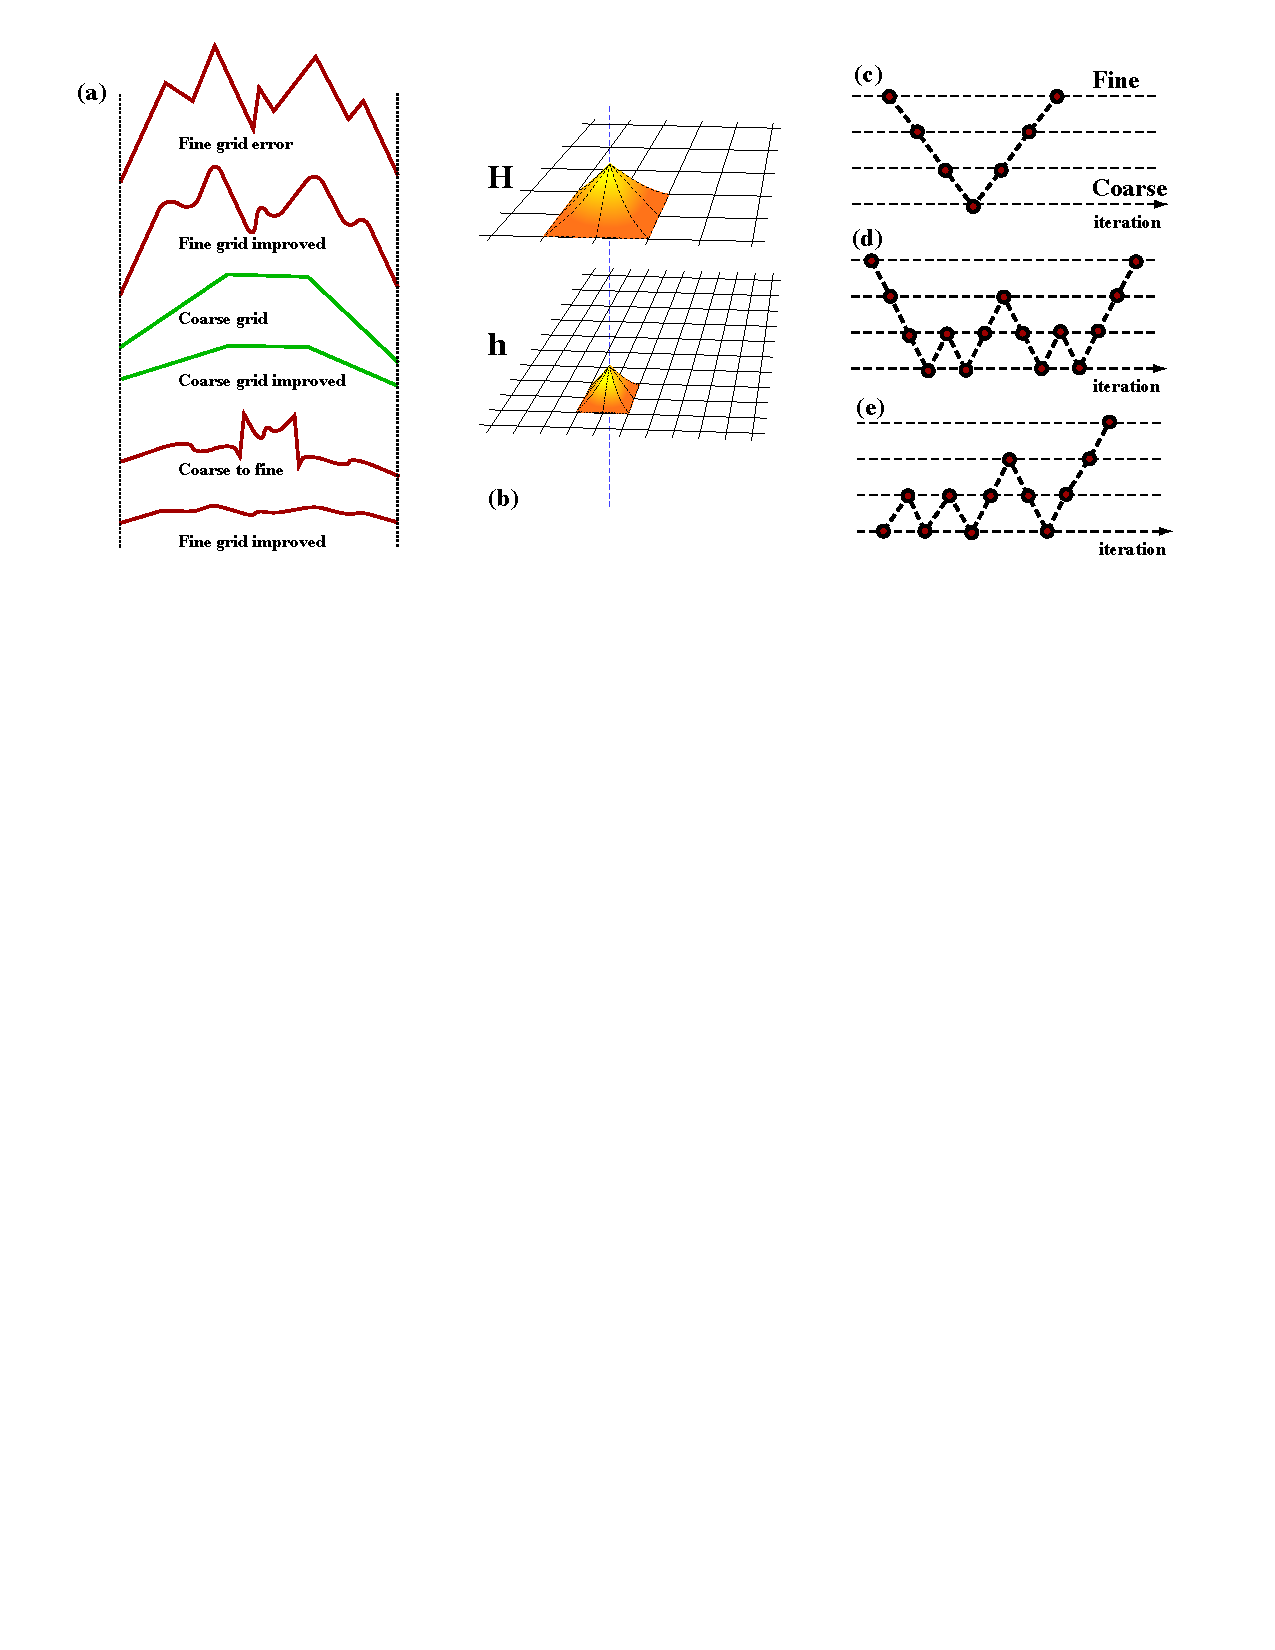
\includegraphics[width=0.66\linewidth]{Diagrams/mg.pdf}
		 			\caption[]{Multigrid: (a) Error reduction during simple two level V cycle,
		 			 (b) Shape functions on different grid scales,
		 			 (c) V cycle on four grids,
		 			 (d) W cycle on four grids,
		 			 (e) Schematic of Full Multigrid V cycles}
		 			\label{fig:mg1}
		 		\end{center}
			\end{figure}	
	
	The multigrid method works by formulating the finite element problem
	on a number of different scales - usually a set of grids which are nested
	one within the other sharing common nodes (see Figure \ref{fig:mg1}a).  The solution 
	progresses on all of the grids at the same time with each grid eliminating
	errors at a different scale. The effect is to propogate information very 
	rapidly between different nodes in the grid which would otherwise be
	prevented by the local support of the element shape functions. In fact,
	by a single traverse from fine to coarse grid and back, all nodes in the mesh 
	can be directly connected to every other -- allowing nodes which are physically
	coupled but remote in the mesh to communicate directly during each iteration
	cycle. 

	The multigrid effect relies upon using an iterative solver on each
	of the grid resolutions which acts like a smoother on the residual
	error at the characteristic scale of that particular grid. People commonly use
	Gauss-Seidel iteration because it has exactly this property. On the coarsest
	grid it is possible to use a direct solver because the number of elements
	is usually very small.

	For an elliptic operator such as the Laplacian of the Stokes' problem 
	encountered in the algorithm above the discretized problem is now written
		\begin{equation}
		  {\bf K}_h {\bf d}_h = {\bf f}_h
		\end{equation}
	where  the $h$ subscript indicates that the problem has been discretized
	to a mesh of fineness $h$.  As before an initial estimate of the velocity
	can be improved by determining the solution to
		\begin{equation}
		  {\bf K}_h \delta {\bf d}_h = {\bf r}_h
		\end{equation}
	where ${\bf r}_h$ is the residual on this mesh, and
	$\delta {\bf d}$ is a correction to $\bf d$ which reduces $\bf r$.
	 In the iterative methods
	described above, the initial approximation and the correction are found
	by solving a simplified version of the problem at the same gridpoints
	in such a way that computation time is reduced dramatically.
	However, another approach to the problem is to obtain an approximate
	solution by solving the problem on a more coarse grid. The reduction
	of the number of degrees of freedom also leads to a more manageable
	problem which can be solved fast. The correction term is therefore:
		\begin{equation}
		  {\bf K}_H \delta{\bf d}_H = {\bf r}_H
		\end{equation}
	where $H$ indicates a coarser level of discretization. The residual
	on the coarser mesh is determined by the use of a projection (restriction)
	operator:
		\begin{equation}
		  {\bf r}_H = {\bf P}_H^h {\bf r}_h
		\end{equation}
	and the approximate solution is then interpolated from the coarse
	to fine grid using an interpolation operator:
		\begin{equation}
		  \delta{\bf d}_h = {\bf I}_H^h \delta{\bf d}_H
		\end{equation}
	The power of the algorithm is in a recursive application. The 
	coarse grid correction is also calculated through the use of a
	still-coarser grid and so on, until the problem is so small
	that an exact solution can be obtained very rapidly.
	
	One very simple, but instructive, algorithm for hierarchical
	residual reduction is the sawtooth cycle (the same logical layout
	as the V cycle of Figure \ref{fig:mg1}c).
	
		\begin{tabbing}
			  xxxxxx \= xxxxxxxx \= xxxxxxx \kill  \\ 
			  $\bullet$ Obtain approximate solution, ${\bf d}_h$ at highest level $h$\\
			  $\bullet$ Calculate residual: ${\bf r}_h = {\bf f}_h - {\bf K}_h {\bf d}_h$\\
			  $\bullet$ Project residual by N levels to level $h-N$\\
			  \> ${\bf r}_{h-i} = {\bf  P}_{h-i}^{h-i+1} {\bf r}_{h-i+1}$\\
			  $\bullet$ Solve exactly: $\delta {\bf u}_{h-N} = {\bf A}_{h-N} {\bf r}_{h-N}$\\
			  $\bullet$ Interpolation steps:\\
			  \> ${\bf r}_{h-i+1} += {\bf I}_{h-i}^{h-i+1} {\bf K}_{h-i} \delta {\bf d}_{h-i} $\\
			  \> Improve $\delta {\bf d}_{h-i+1}$ \\
			  $\bullet$ ${\bf d}_h += \delta {\bf d}_h$\\
		\end{tabbing}
	
	The step in which the velocity correction is ``improved'' is an iterative
	method for reducing the residual at the current level such as those described
	above. Although many methods of residual reduction are available, the class
	of methods which work best with the multigrid approach are relaxation iterations
	which are also effective {\sl smoothing} operators. At each level the smoothing
	operators reduce the residual most strongly on the scale  of the discretization --
	the hierarchical nesting of different mesh sizes allows the residual to be reduced
	at each scale very efficiently. (see Parsons and Hall).  The Jacobi relaxation
	above is a suitable algorithm for multigrid enhancement but still converges too
	slowly to build into an efficient code. Preconditioned conjugate gradient
	methods can better reduce the residual for the same number of operations
	but may not possess the smoothing properties which benefit the multigrid
	approach. The local inverse method appears to have both the smoothing and 
	rapid convergence properties for the Stokes' problem which are required for
	effective multigridding.
	
	The projection and interpolation operators have to be chosen fairly carefully
	to avoid poor approximations to the problem at the coarse levels and ineffectual
	corrections propogated to the fine levels. The interpolation operator is defined 
	naturally from the shape functions at the coarse levels. The projection operator
	is then defined to complement this choice (the operators should be adjoint).
	
	The sawtooth cycle given in this section is the simplest multigrid algorithm.
	Developments include improving the residual at each level of the {\sl projection},
	known as a `v-cycle', and cycles in which the residual is interpolated only part
	way through the hierarchy before being reprojected and subjected to another
	set of improvements (a `w-cycle'). 
	
	The Full Multigrid Algorithm (see Brandt) introduces a further level of complexity.
	Instead of simply casting the problem at a single level and projecting/improving
	the residual on a number of grids, the whole problem is defined for all the grids.
	In this way the initial fine-grid approximation is obtained by interpolating
	from the solution to the coarsest grid problem. The solution at each level
	is still obtained by projecting to the finest level and reducing
	the residual at each projection step. The result is some sort of 
	``Loch Ness Monster'' cycle.
	
	One of the major problems in multigrid is knowing how best to represent
	material properties at different levels of grid coarseness in order to 
	obtain the optimal convergence rate. This has a simple solution in
	the particle in cell finite element methods which we will discuss later.

\section{A Practical Mixed Formulation}

	The fact that the mixed method does not provide a positive definite matrix is
	a potentially serious difficulty. It can be avoided by the following rearrangement.
	
	Multiplying out the mixed method equations gives the conservation
	equations for momentum and mass
	
	\begin{subequations}
		  \begin{equation}
			    {\bf Kd} + {\bf G}^T{\bf p} = {\bf f} 
			    \label{eq:stokes}
		  \end{equation}
		  \begin{equation}
			    {\bf Gd} = {\bf 0}
		  \end{equation}
	\end{subequations}

	
	Multiply equation (\ref{eq:stokes}) throughout by $ {\bf G}{\bf K}^{-1}$
	to give
	\begin{equation}
		{\bf Gd} + {\bf G K}^{-1}{\bf G}^T {\bf p} = {\bf G K}^{-1}{\bf  f}
	\end{equation}
	where the first term is zero due to the incompressibility condition.
	Then the equation system is in the form $\hat{\bf K}{\bf p} = \hat{\bf f}$, where
	$\hat{\bf K}$ is  now positive definite, and so a conjugate
	gradient method can be used:
	
	\begin{tabbing}
	  xxxxxx \= xxxxxxxx \= xxxxxxx \kill 
	  $ k = 0; {\bf p}_0 = {\bf 0}; {\bf r}_0 = \hat{\bf f}$ \\
	  {\tt while} $({\bf r}_k \not= {\bf 0})$ \\
	  \> $ k = k + 1 $\\
	  \> {\tt if} $(k=1)$ \\
	  \> \>$ {\bf s}_1 = {\bf r}_0$\\
	  \> {\tt else} \\
	  \> \> $\beta = ({\bf r}_{k-1},{\bf r}_{k-1})/({\bf r}_{k-2},{\bf r}_{k-2})$\\
	  \> \> ${\bf s}_k = {\bf r}_{k-1} + \beta {\bf s}_{k-1}$\\
	  \> {\tt end}\\
	  \> ${\bf w} = \hat{\bf K} {\bf s}$\\
	  \> $\alpha = ({\bf r}_{k},{\bf r}_{k})/({\bf s}_{k},{\bf w})$\\
	  \> ${\bf p}_k = {\bf p}_{k-1} + \alpha {\bf s}_{k}$\\
	  \> ${\bf r}_k = {\bf r}_{k-1} - \alpha {\bf w}$\\
	  {\tt end}\\
	  ${\bf d} = {\bf d}_k$
	\end{tabbing}
	
	However, it is not possible to obtain $\hat{\bf K}$ or $\hat{\bf f}$ directly
	because the form of ${\bf K}^{-1}$ is not known --- the reason for the
	use of an iterative method in the first place. In order to obtain the initial
	residual, therefore, perform the following operation,
	\begin{tabbing}
	  xxxxxx \= xxxxxxxx \= xxxxxxx \kill 
	  \> ${\bf r}_0 = {\bf G K}^{-1} {\bf f}$: \\
	  \> solve: ${\bf K d} = {\bf f}$ for $\bf d$\\
	  \> set: ${\bf r}_0 = {\bf G d} = {\bf G K}^{-1} {\bf f}$
	\end{tabbing}
	and to find the $\bf w$ vector:
	\begin{tabbing}
	  xxxxxx \= xxxxxxxx \= xxxxxxx \kill 
	  \> ${\bf w} = \hat{\bf G K}^-1{\bf G}^T {\bf s}$: \\
	  \> solve ${\bf K d} = {\bf G}^T {\bf s}$ for $\bf d$\\
	  \> set ${\bf w} = {\bf K d} = {\bf G K}^{-1}{\bf G}^T {\bf s}$
	\end{tabbing}


\section{Time}

	We have concentrated on the solution to equibrium equations without really
	touching on the way time is evolved in elasticity and slow flow where the 
	equations themselves are independent of time.
	In the mantle dynamics problem, the energy equation contains time derivatives which the equation of
	motion lacks so it is unsurprising that these equations require entirely
	different computational methods.
	
	We almost always want to know the time-history 
	of our simulations, so we generally solve this equation explicitly
	in time. 
	
	Variational methods are not generally applicable because the energy equation with
	its strong advection term does not follow an extremum of some functional. In this
	case even the weak forms of the equation are quite similar to finite difference equations.
	
%\section{Ideas on a Particle in Cell Finite Element Code}
%	
%	The extension of standard finite element
%	methods to include a basic Lagrangian Particle reference
%	frame. 
%	
%	Adapting integration schemes.
%	
%	Problems for highly active flow regimes.
%
%	Discussion: as this is ongoing, research work with 
%	potentially exciting commercial applications, it will be discussed but
%	not written out here !!
%	
%\subsection{Geological Examples from a PIC / FE method}
%
%	To wind down the course, we will watch some movies
%	of finite elements in action.

\end{document}
